%%%%%%%%%%%%%%%%%%%%%%%%%%%%%%%%%%%%%%%%%
% Lachaise Assignment
% LaTeX Template
% Version 1.0 (26/6/2018)
%
% This template originates from:
% http://www.LaTeXTemplates.com
%
% Authors:
% Marion Lachaise & François Févotte
% Vel (vel@LaTeXTemplates.com)
%
% License:
% CC BY-NC-SA 3.0 (http://creativecommons.org/licenses/by-nc-sa/3.0/)
% 
%%%%%%%%%%%%%%%%%%%%%%%%%%%%%%%%%%%%%%%%%

%----------------------------------------------------------------------------------------
%	PACKAGES AND OTHER DOCUMENT CONFIGURATIONS
%----------------------------------------------------------------------------------------

\documentclass{article}

%%%%%%%%%%%%%%%%%%%%%%%%%%%%%%%%%%%%%%%%%
% Lachaise Assignment
% Structure Specification File
% Version 1.0 (26/6/2018)
%
% This template originates from:
% http://www.LaTeXTemplates.com
%
% Authors:
% Marion Lachaise & François Févotte
% Vel (vel@LaTeXTemplates.com)
%
% License:
% CC BY-NC-SA 3.0 (http://creativecommons.org/licenses/by-nc-sa/3.0/)
% 
%%%%%%%%%%%%%%%%%%%%%%%%%%%%%%%%%%%%%%%%%

%----------------------------------------------------------------------------------------
%	PACKAGES AND OTHER DOCUMENT CONFIGURATIONS
%----------------------------------------------------------------------------------------

\usepackage{amsmath,amsfonts,stmaryrd,amssymb} % Math packages

\usepackage{enumerate} % Custom item numbers for enumerations

\usepackage[ruled]{algorithm2e} % Algorithms

\usepackage[framemethod=tikz]{mdframed} % Allows defining custom boxed/framed environments

\usepackage{listings} % File listings, with syntax highlighting
\lstset{
	basicstyle=\ttfamily, % Typeset listings in monospace font
}

\usepackage[ampersand]{easylist}

\usepackage{subcaption}

\ListProperties(Hide=100, Hang=true, Progressive=3ex, Style*=-- ,
Style2*=$\bullet$ ,Style3*=$\circ$ ,Style4*=\tiny$\blacksquare$ )

%----------------------------------------------------------------------------------------
%	DOCUMENT MARGINS
%----------------------------------------------------------------------------------------

\usepackage{geometry} % Required for adjusting page dimensions and margins

\geometry{
	paper=a4paper, % Paper size, change to letterpaper for US letter size
	top=2.5cm, % Top margin
	bottom=3cm, % Bottom margin
	left=2.5cm, % Left margin
	right=2.5cm, % Right margin
	headheight=14pt, % Header height
	footskip=1.5cm, % Space from the bottom margin to the baseline of the footer
	headsep=1.2cm, % Space from the top margin to the baseline of the header
	%showframe, % Uncomment to show how the type block is set on the page
}

%----------------------------------------------------------------------------------------
%	FONTS
%----------------------------------------------------------------------------------------

\usepackage[utf8]{inputenc} % Required for inputting international characters
\usepackage[T1]{fontenc} % Output font encoding for international characters

\usepackage{XCharter} % Use the XCharter fonts

%----------------------------------------------------------------------------------------
%	COMMAND LINE ENVIRONMENT
%----------------------------------------------------------------------------------------

% Usage:
% \begin{commandline}
%	\begin{verbatim}
%		$ ls
%		
%		Applications	Desktop	...
%	\end{verbatim}
% \end{commandline}

\mdfdefinestyle{commandline}{
	leftmargin=10pt,
	rightmargin=10pt,
	innerleftmargin=15pt,
	middlelinecolor=black!50!white,
	middlelinewidth=2pt,
	frametitlerule=false,
	backgroundcolor=black!5!white,
	frametitle={Command Line},
	frametitlefont={\normalfont\sffamily\color{white}\hspace{-1em}},
	frametitlebackgroundcolor=black!50!white,
	nobreak,
}

% Define a custom environment for command-line snapshots
\newenvironment{commandline}{
	\medskip
	\begin{mdframed}[style=commandline]
}{
	\end{mdframed}
	\medskip
}

%----------------------------------------------------------------------------------------
%	FILE CONTENTS ENVIRONMENT
%----------------------------------------------------------------------------------------

% Usage:
% \begin{file}[optional filename, defaults to "File"]
%	File contents, for example, with a listings environment
% \end{file}

\mdfdefinestyle{file}{
	innertopmargin=1.6\baselineskip,
	innerbottommargin=0.8\baselineskip,
	topline=false, bottomline=false,
	leftline=false, rightline=false,
	leftmargin=2cm,
	rightmargin=2cm,
	singleextra={%
		\draw[fill=black!10!white](P)++(0,-1.2em)rectangle(P-|O);
		\node[anchor=north west]
		at(P-|O){\ttfamily\mdfilename};
		%
		\def\l{3em}
		\draw(O-|P)++(-\l,0)--++(\l,\l)--(P)--(P-|O)--(O)--cycle;
		\draw(O-|P)++(-\l,0)--++(0,\l)--++(\l,0);
	},
	nobreak,
}

% Define a custom environment for file contents
\newenvironment{file}[1][File]{ % Set the default filename to "File"
	\medskip
	\newcommand{\mdfilename}{#1}
	\begin{mdframed}[style=file]
}{
	\end{mdframed}
	\medskip
}

%----------------------------------------------------------------------------------------
%	NUMBERED QUESTIONS ENVIRONMENT
%----------------------------------------------------------------------------------------

% Usage:
% \begin{question}[optional title]
%	Question contents
% \end{question}

\mdfdefinestyle{question}{
	innertopmargin=1.2\baselineskip,
	innerbottommargin=0.8\baselineskip,
	roundcorner=5pt,
	nobreak,
	singleextra={%
		\draw(P-|O)node[xshift=1em,anchor=west,fill=white,draw,rounded corners=5pt]{%
		Question \theQuestion\questionTitle};
	},
}

\newcounter{Question} % Stores the current question number that gets iterated with each new question

% Define a custom environment for numbered questions
\newenvironment{question}[1][\unskip]{
	\bigskip
	\stepcounter{Question}
	\newcommand{\questionTitle}{~#1}
	\begin{mdframed}[style=question]
}{
	\end{mdframed}
	\medskip
}

%----------------------------------------------------------------------------------------
%	WARNING TEXT ENVIRONMENT
%----------------------------------------------------------------------------------------

% Usage:
% \begin{warn}[optional title, defaults to "Warning:"]
%	Contents
% \end{warn}

\mdfdefinestyle{warning}{
	topline=false, bottomline=false,
	leftline=false, rightline=false,
	nobreak,
	singleextra={%
		\draw(P-|O)++(-0.5em,0)node(tmp1){};
		\draw(P-|O)++(0.5em,0)node(tmp2){};
		\fill[black,rotate around={45:(P-|O)}](tmp1)rectangle(tmp2);
		\node at(P-|O){\color{white}\scriptsize\bf !};
		\draw[very thick](P-|O)++(0,-1em)--(O);%--(O-|P);
	}
}

% Define a custom environment for warning text
\newenvironment{warn}[1][Warning:]{ % Set the default warning to "Warning:"
	\medskip
	\begin{mdframed}[style=warning]
		\noindent{\textbf{#1}}
}{
	\end{mdframed}
}

%----------------------------------------------------------------------------------------
%	INFORMATION ENVIRONMENT
%----------------------------------------------------------------------------------------

% Usage:
% \begin{info}[optional title, defaults to "Info:"]
% 	contents
% 	\end{info}

\mdfdefinestyle{info}{%
	topline=false, bottomline=false,
	leftline=false, rightline=false,
	nobreak,
	singleextra={%
		\fill[black](P-|O)circle[radius=0.4em];
		\node at(P-|O){\color{white}\scriptsize\bf i};
		\draw[very thick](P-|O)++(0,-0.8em)--(O);%--(O-|P);
	}
}

% Define a custom environment for information
\newenvironment{info}[1][Info:]{ % Set the default title to "Info:"
	\medskip
	\begin{mdframed}[style=info]
		\noindent{\textbf{#1}}
}{
	\end{mdframed}
}
 % Include the file specifying the document structure and custom commands

%----------------------------------------------------------------------------------------
%	ASSIGNMENT INFORMATION
%----------------------------------------------------------------------------------------

\title{Starbucks Capstone Project Report} % Title of the assignment

\author{Egor Makhov\\ \texttt{george.mahoff@gmail.com}} % Author name and email address

\date{Udacity, MLE Nanodegree --- \today} % University, school and/or department name(s) and a date

%----------------------------------------------------------------------------------------

\begin{document}

\maketitle % Print the title

%----------------------------------------------------------------------------------------
%	INTRODUCTION
%----------------------------------------------------------------------------------------

\section*{Domain background}
This Starbucks Capstone project is part of the Udacity Machine Learning Engineer Nanodegree. Udacity partnered with Starbucks to provide a real-world business problem and simulated data mimicking their customer behaviour.

Starbucks is an American coffeehouse chain. Once every few days, Starbucks sends out an offer to users via different ways such as mobile app. An offer can be merely an advertisement for a drink or an actual offer such as a discount or BOGO (buy one get one free). Some users might not receive any offer during certain weeks. An important characteristic regarding this capstone is that not all users receive the same offer. As part of marketing strategy, we always want to figure out if a customer will spend more by giving a sound offer. Providing right offer to right customer could help build loyalty of the brand and product and as a result increasing sales margins in the long run

\section*{Problem statement}

The problem we are looking to solve here is conceptually easy to understand, albeit difficult to answer. We are looking to best determine which kind of offer to send to each customer segment based on their purchasing decisions. We’ll touch more on what these offers are and data we’ll be utilizing down in the next section. We will leverage traditional evaluation metrics to determine which model is most appropriate for our dataset. These evaluation metrics will be discussed in an upcoming section.

\section*{Datasets and inputs}

As given by the Udacity’s Starbucks Project Overview:\newline

\begin{easylist}
&& The program used to create the data simulates how people make purchasing decisions and how those decisions are influenced by promotional offers.
&& Each person in the simulation has some hidden traits that influence their purchasing patterns and are associated with their observable traits. People produce various events, including receiving offers, opening offers, and making purchases.
&& As a simplification, there are no explicit products to track. Only the amounts of each transaction or offer are recorded.
&& There are three types of offers that can be sent: buy-one-get-one (BOGO), discount, and informational. In a BOGO offer, a user needs to spend a certain amount to get a reward equal to that threshold amount. In a discount, a user gains a reward equal to a fraction of the amount spent. In an informational offer, there is no reward, but neither is there a requisite amount that the user is expected to spend. Offers can be delivered via multiple channels.
&& The basic task is to use the data to identify which groups of people are most responsive to each type of offer, and how best to present each type of offer.\newline
\end{easylist}
\newpage
\noindent The data is divided in 3 files:\newline

\begin{easylist}
& profile.json: Rewards program users (17000 users x 5 fields)
&& gender: (categorical) M, F, O, or null
&& age: (numeric) missing value encoded as 118
&& id: (string/hash)
&& became\_member\_on: (date) format YYYYMMDD 
&& income: (numeric)\newline

& portfolio.json: Offers sent during 30-day test period (10 offers x 6 fields)
&& reward: (numeric) money awarded for the amount spent
&& channels: (list) web, email, mobile, social
&& difficulty: (numeric) money required to be spent to receive reward
&& duration: (numeric) time for offer to be open, in days
&& offer\_type: (string) bogo, discount, informational
&& id: (string/hash)\newline

& transcript.json: Event log (306648 events x 4 fields)
&& person: (string/hash)
&& event: (string) offer received, offer viewed, transaction, offer completed
&& value: (dictionary) different values depending on event type
&& offer id: (string/hash) not associated with any “transaction”
&& amount: (numeric) money spent in “transaction”
&& reward: (numeric) money gained from “offer completed”
&& time: (numeric) hours after start of test
\end{easylist}

% -----------------------------------------
\section*{Data cleaning}

\subsection*{Portfolio Dataset}
\begin{easylist}
&& One-Hot Encode the channels column.
&& One-Hot Encode the offer\_type column.
&& Rename id to id\_offer.
&& Reorder columns so id\_offer is first, for display purposes only.
\end{easylist}

\begin{figure}[h]
  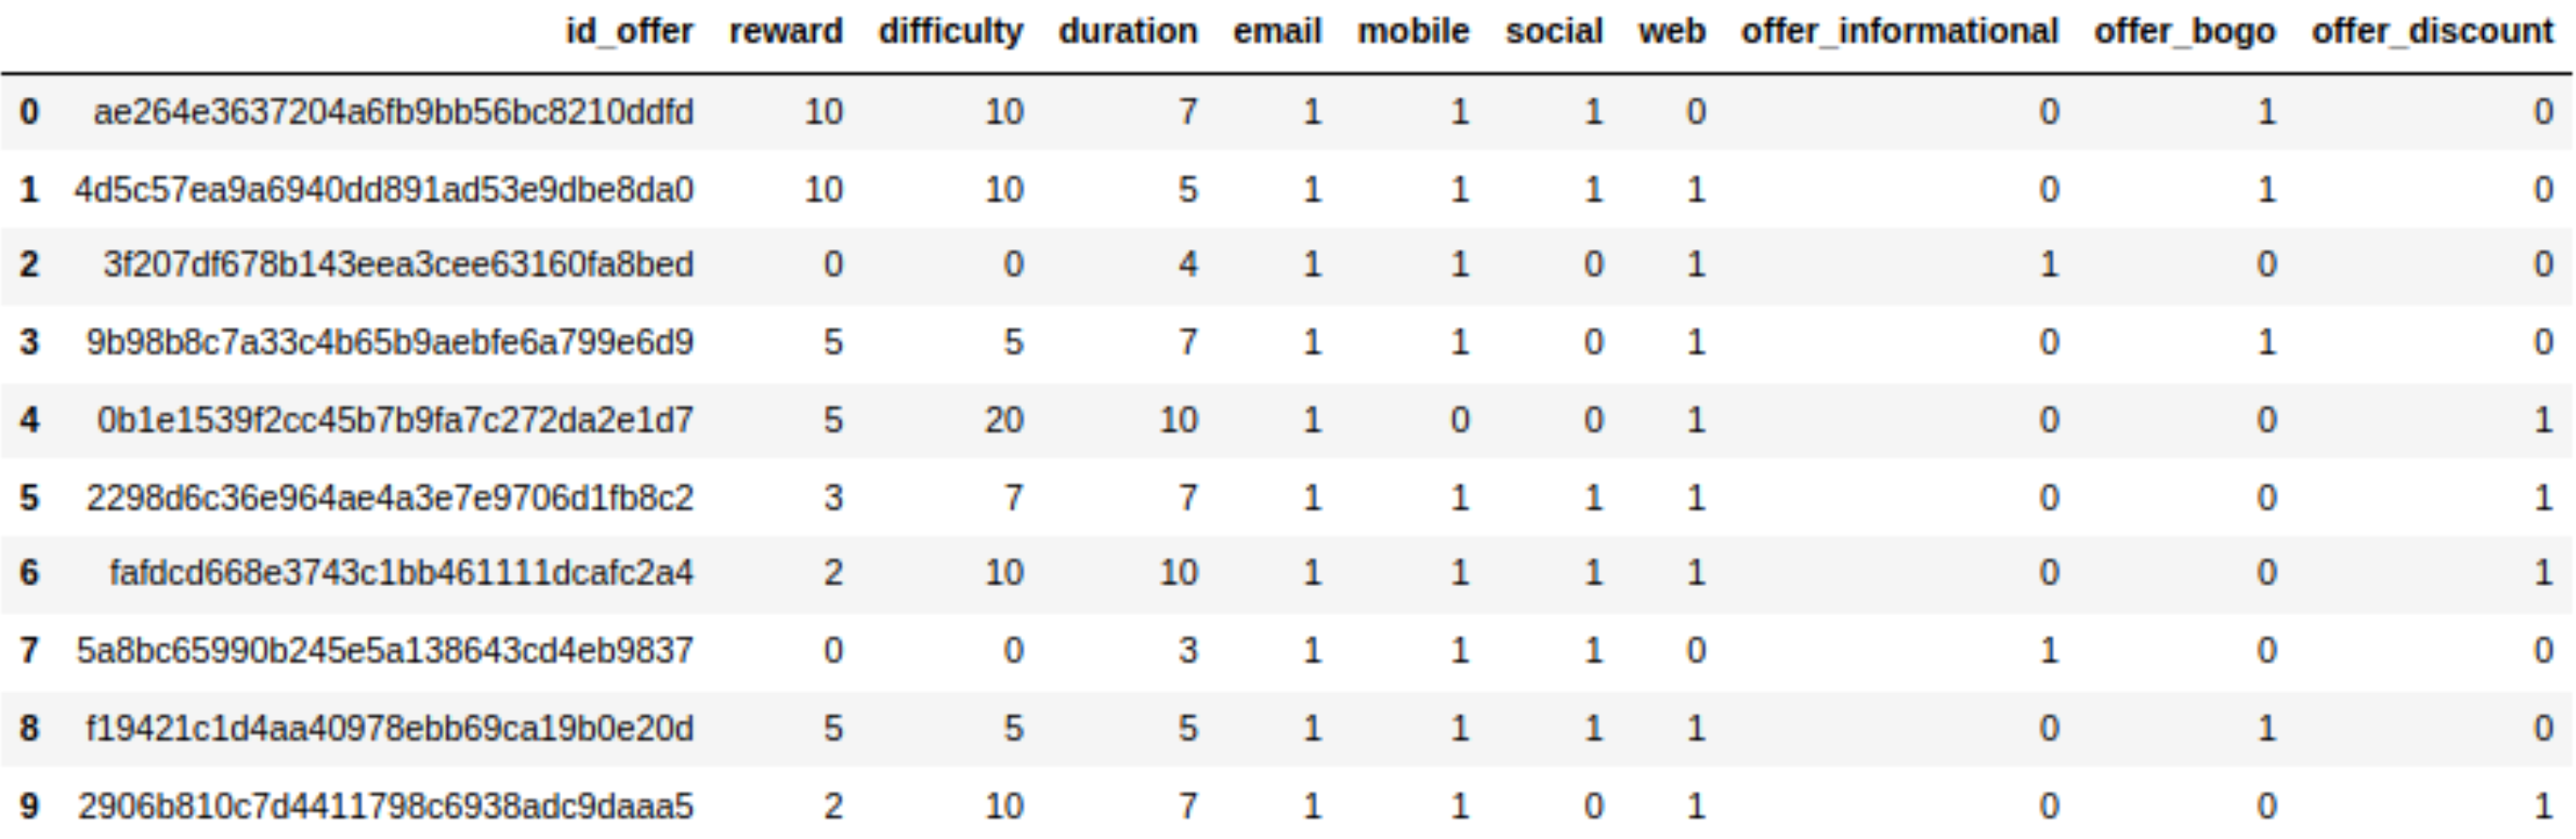
\includegraphics[width=\linewidth]{img/01.png}
  \caption{Complete Portfolio after cleaning}
  \label{fig:01}
\end{figure}

\subsection*{Profile Dataset}
\begin{easylist}
&& Remove customers with missing data (gender is None, age is 118, and income is NaN). I verified that whenever a customer left one of these optional fields blank, they left all three of them blank.
&& Calculate number of days the customer has been a member.
&& Store the year the customer became a member on (temporarily for graphing purposes).
&& One-Hot Encode the customer’s age into buckets by decade (10 to 19, 20 to 29, 30 to 39, etc.)
&& One-Hot Encode the customer’s gender.
&& Rename id to id\_customer.
&& Reorder columns so id\_customer is first, for display purposes only.
\end{easylist}

\begin{figure}[h]
  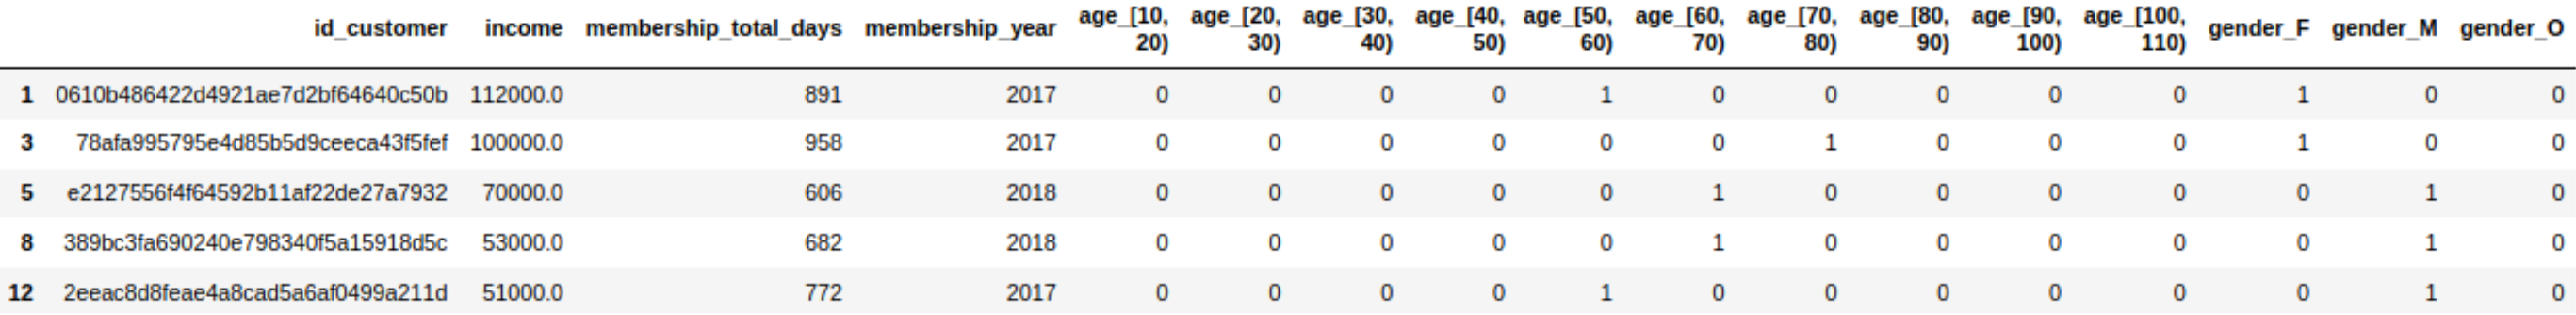
\includegraphics[width=\linewidth]{img/02.png}
  \caption{First 5 rows of cleaned Profile}
  \label{fig:02}
\end{figure}

\subsection*{Transcript Dataset}
\begin{easylist}
&& Rename person to id\_customer.
&& One-Hot Encode events.
&& Get ‘offer id’ from value column dictionary and place in new column id\_offer.
&& Get ‘amount’ from value column dictionary and place in new column trans\_amt.
\end{easylist}

\begin{figure}[h]
  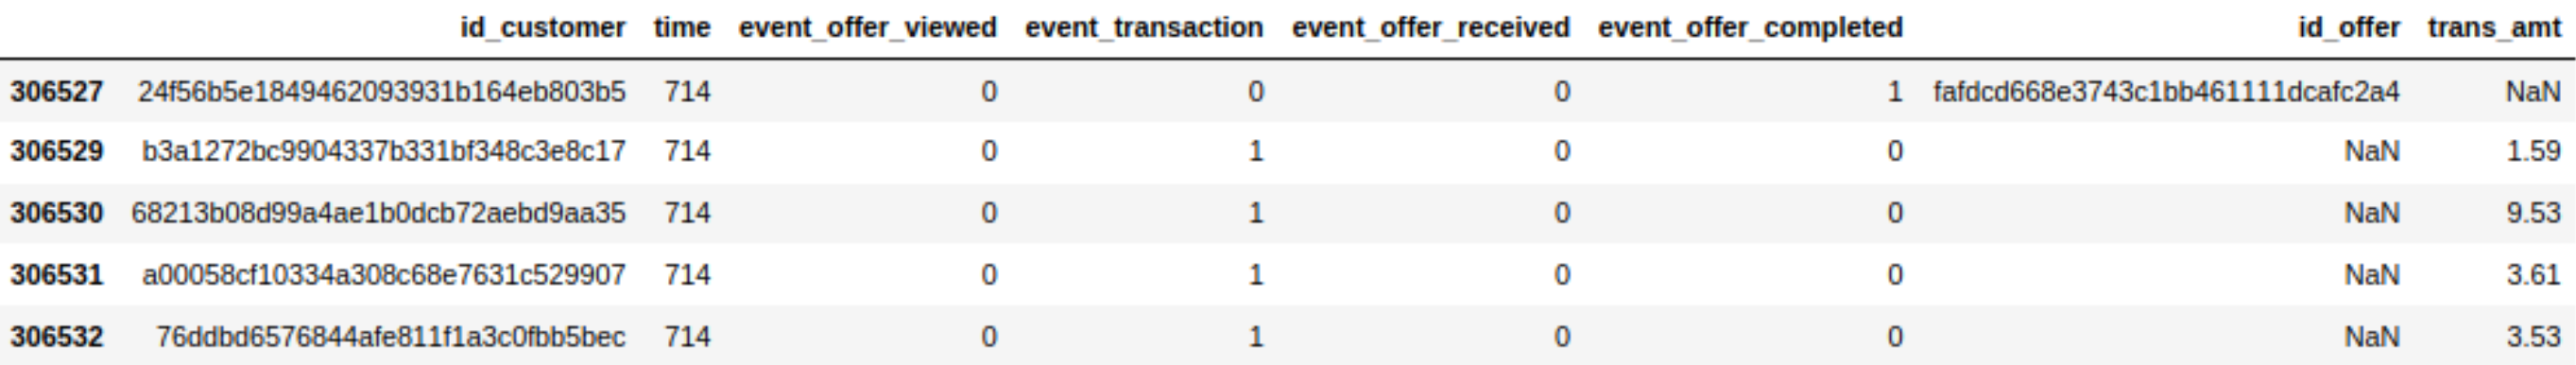
\includegraphics[width=\linewidth]{img/03.png}
  \caption{Last 5 rows of cleaned Transcript}
  \label{fig:03}
\end{figure}

% -----------------------------------------
\section*{Preliminary data analysis}

Key points observed when exploring the data:\newline
\begin{easylist}
& Portfolio dataset exploration
&& Every offer was sent via the email channel, in addition to other channels.
&& Informational offer types are never “completed” since they have no difficulty.\newline

& Profile dataset exploration
&& The three optional fields for users when creating a profile are gender, age, and income. I was concerned that customers may have provided some information but left other fields default (ex: they enter gender and age but leave income default). I verified that the whenever a field was left default, they were all left default. There are 2175 customers that left these optional fields default.
&& The youngest customer age is 18. The oldest actual customer age (not the default 118) is 101 years old.
&& The earliest membership is July 29, 2013 and the most recent membership is July 26, 2018.\newline
 
\begin{figure}[ht!]
\begin{subfigure}{0.5\textwidth}
	\label{sfig:04}
    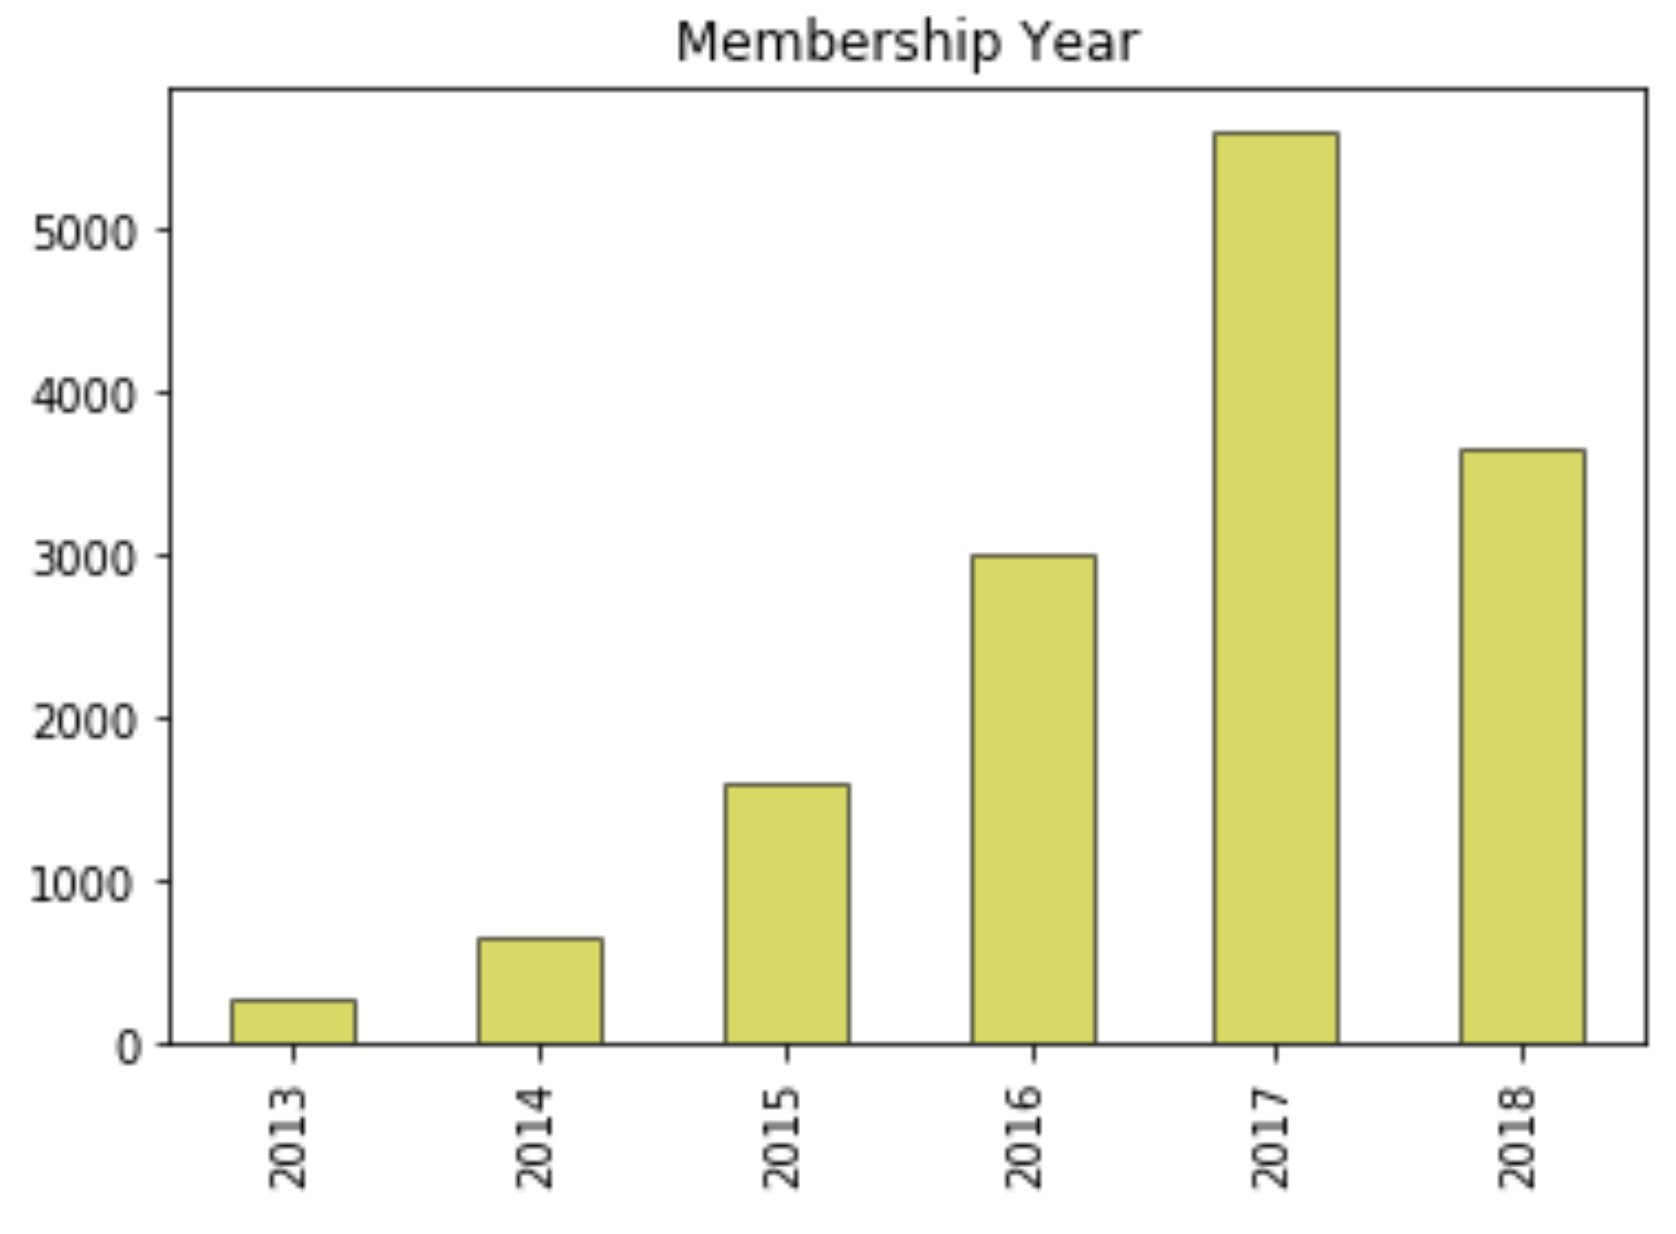
\includegraphics[width=0.9\textwidth, height=7cm]{img/04.png}
    \caption{Profile Memberships Per Year}
\end{subfigure}
\begin{subfigure}{0.5\textwidth}
	\label{sfig:05}
    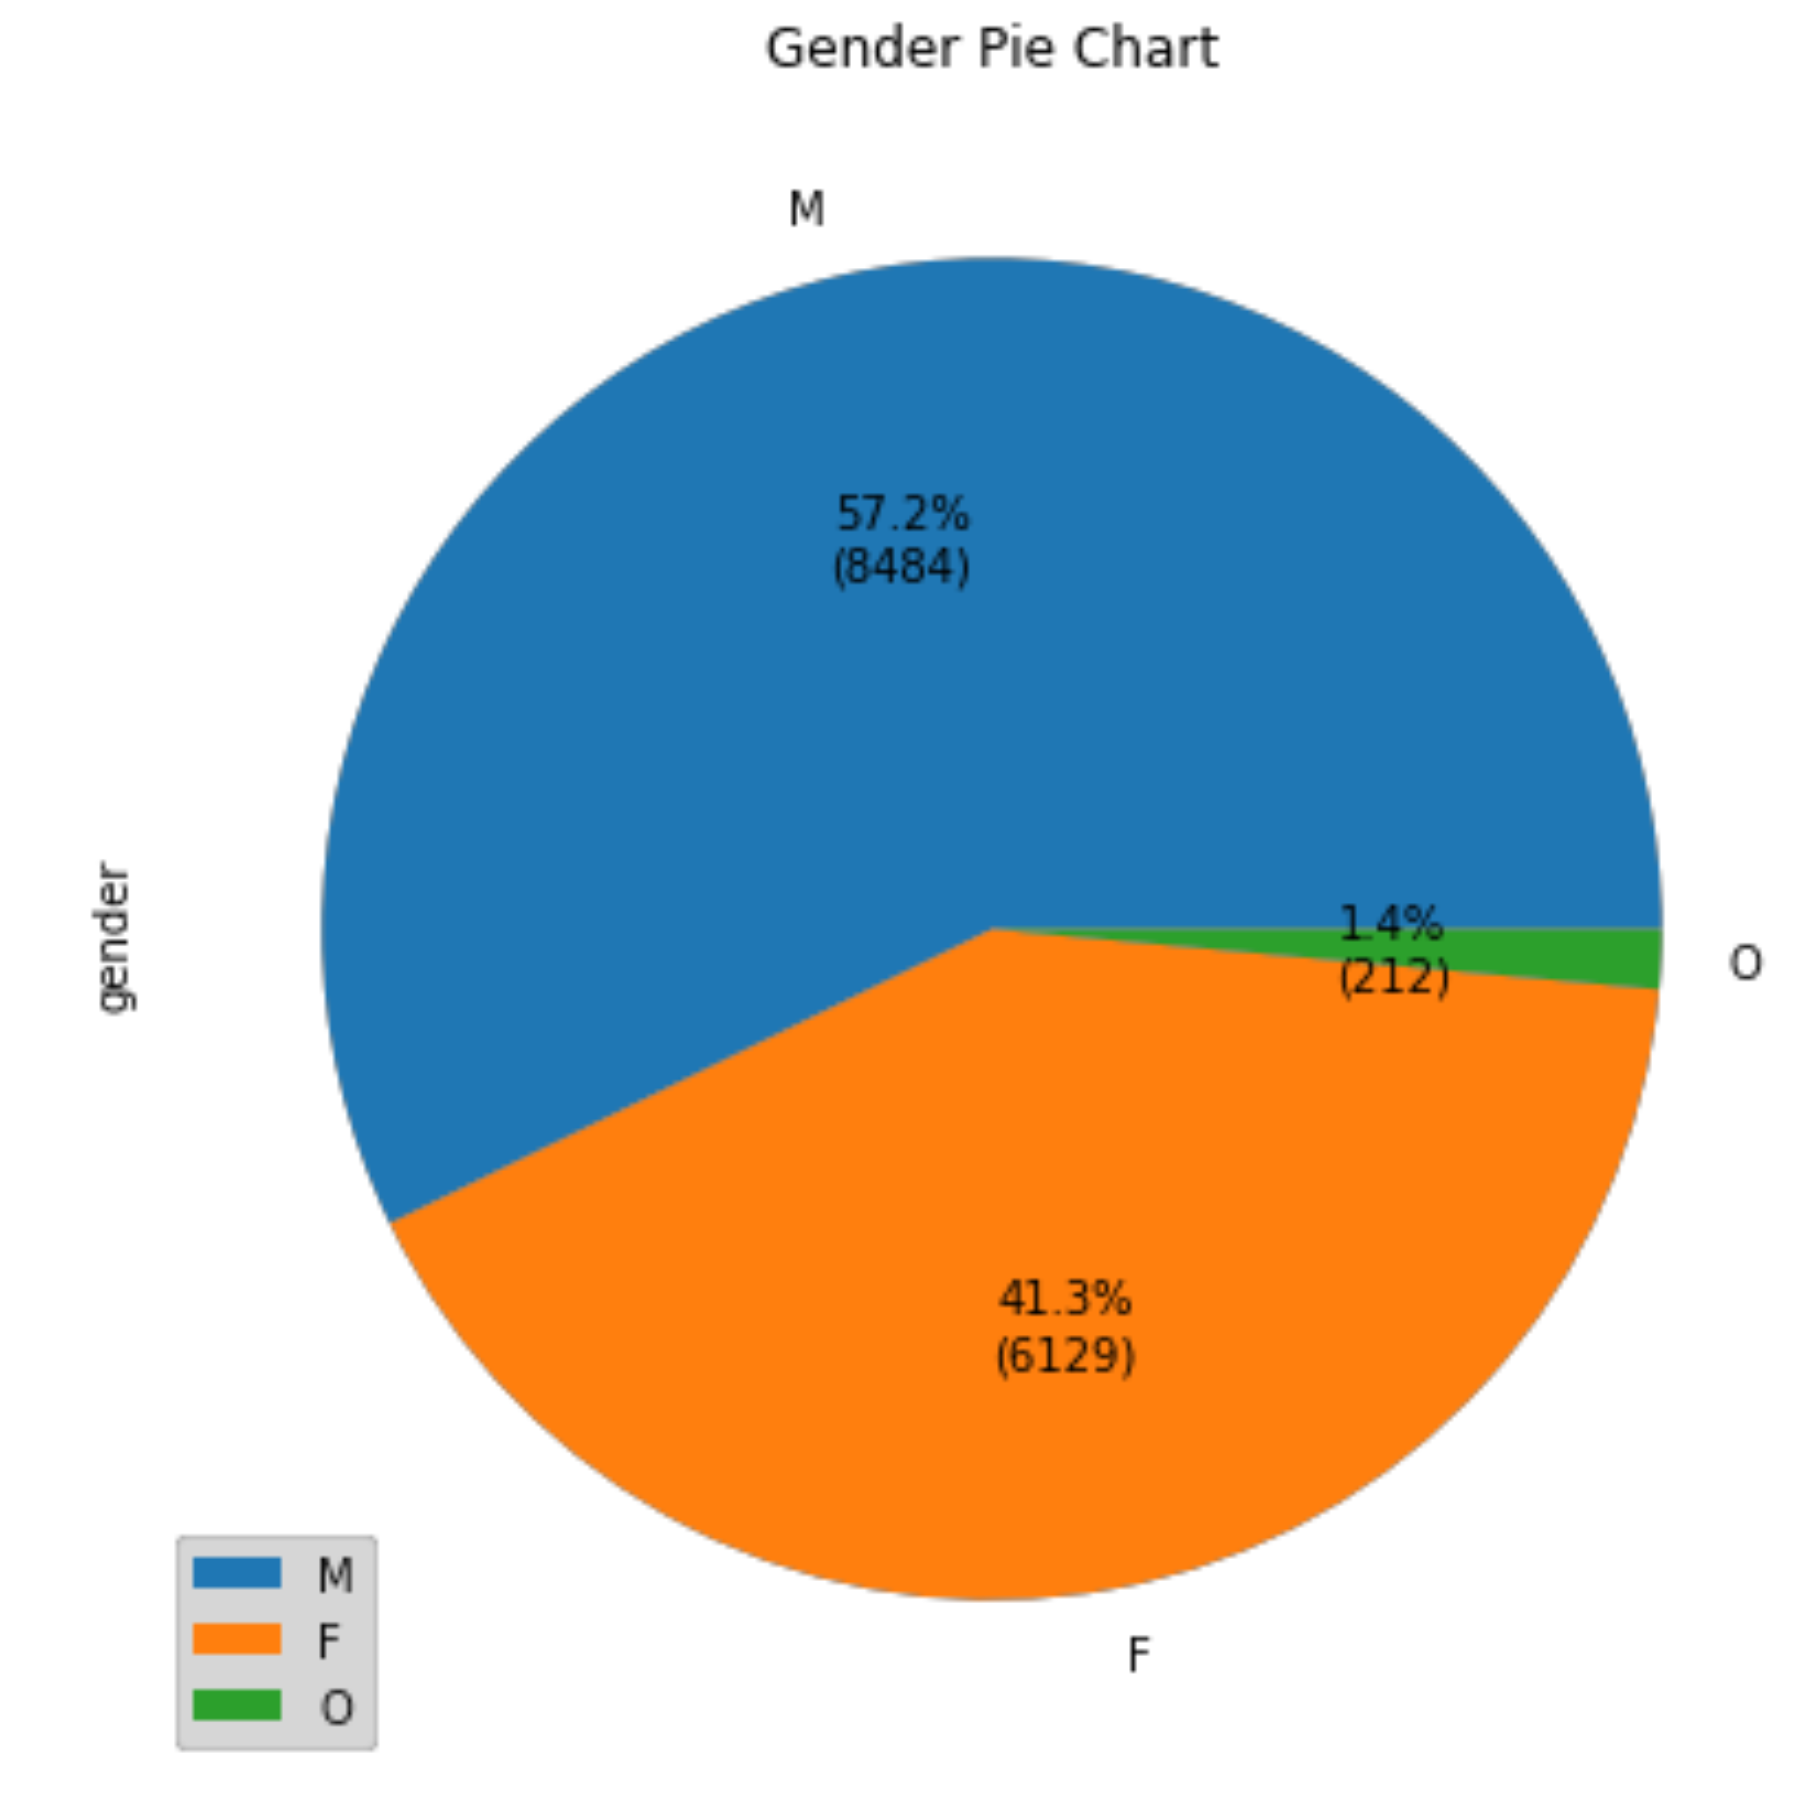
\includegraphics[width=0.9\textwidth, height=7cm]{img/05.png}
    \caption{Profile Gender Percentages and Counts}
\end{subfigure}
\begin{subfigure}{0.5\textwidth}
	\label{sfig:06}
    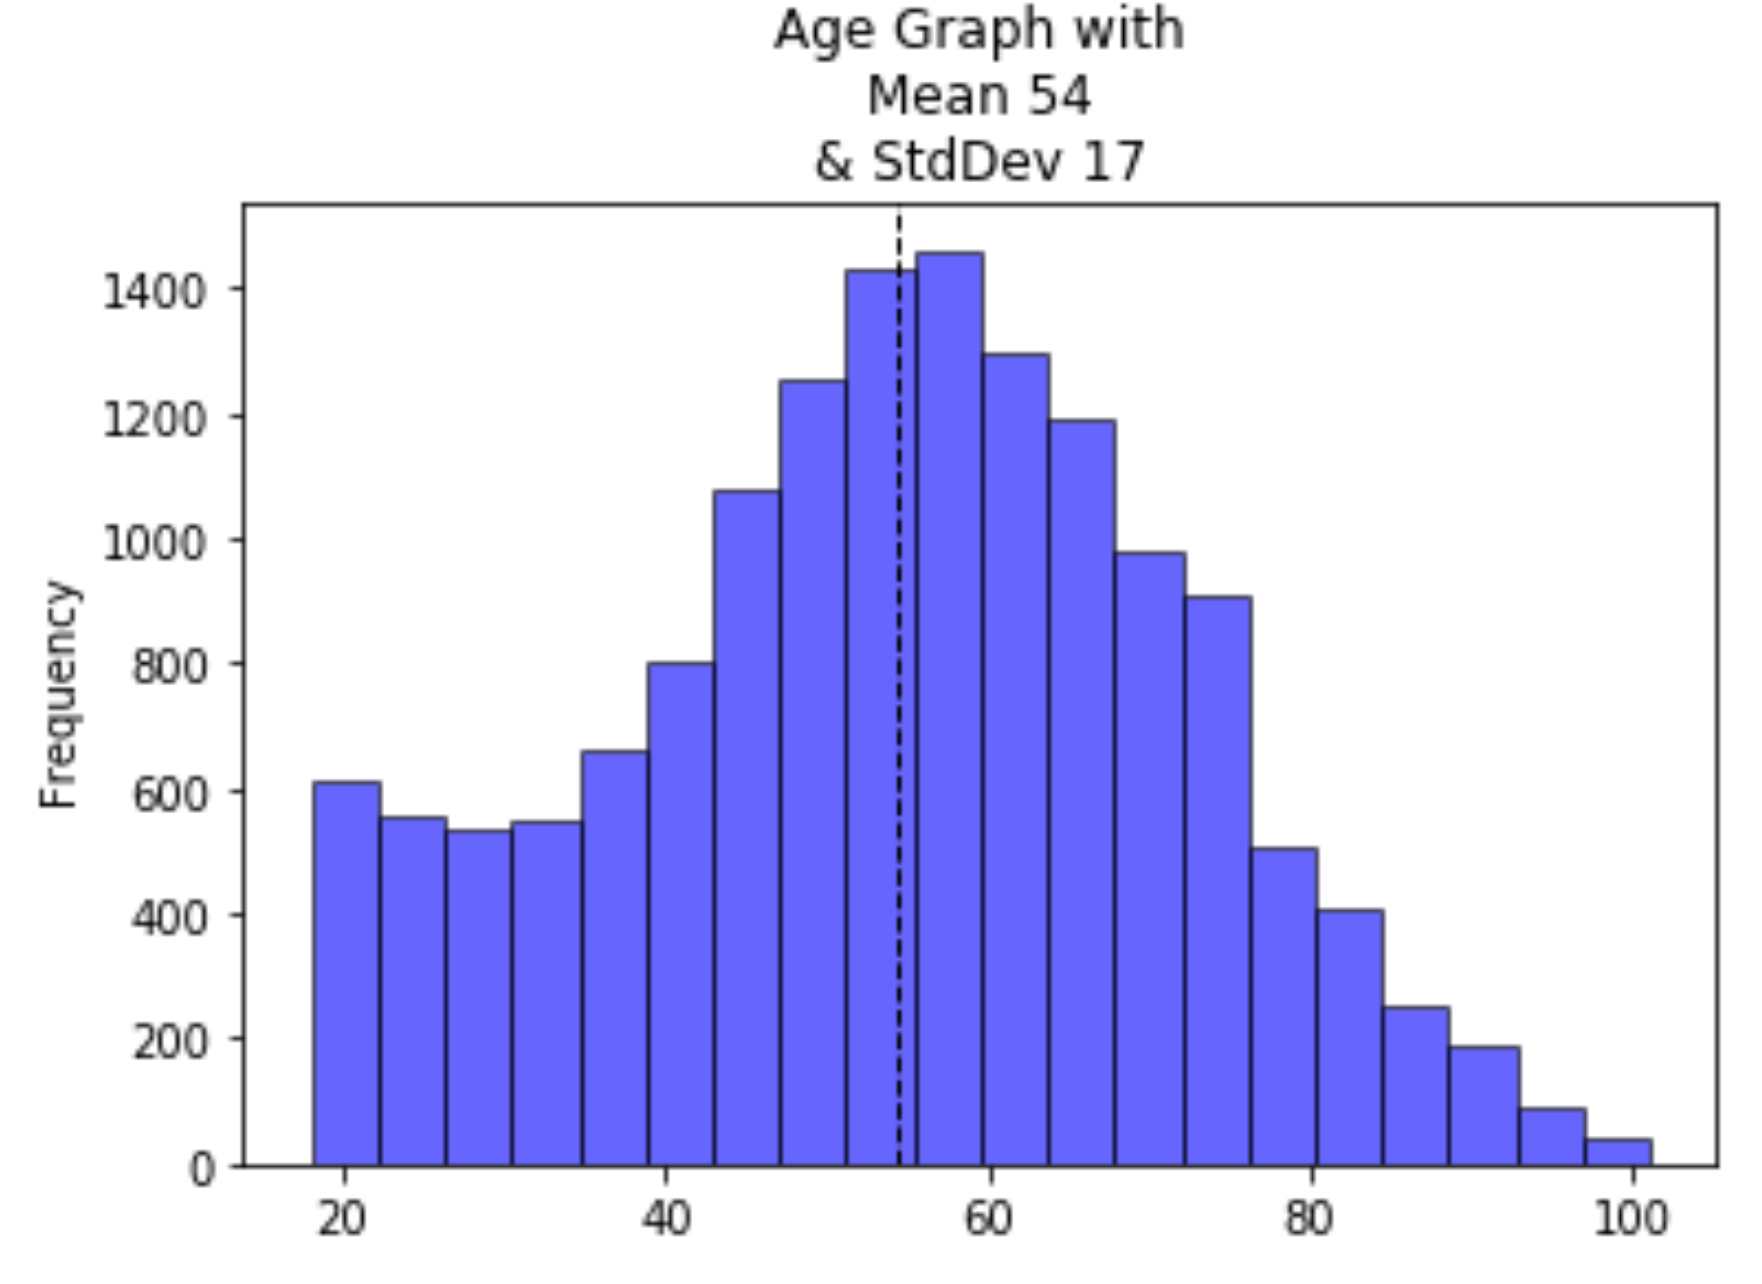
\includegraphics[width=0.9\textwidth, height=7cm]{img/06.png}
    \caption{Profile Age Distribution}
\end{subfigure}
\begin{subfigure}{0.5\textwidth}
	\label{sfig:07}
    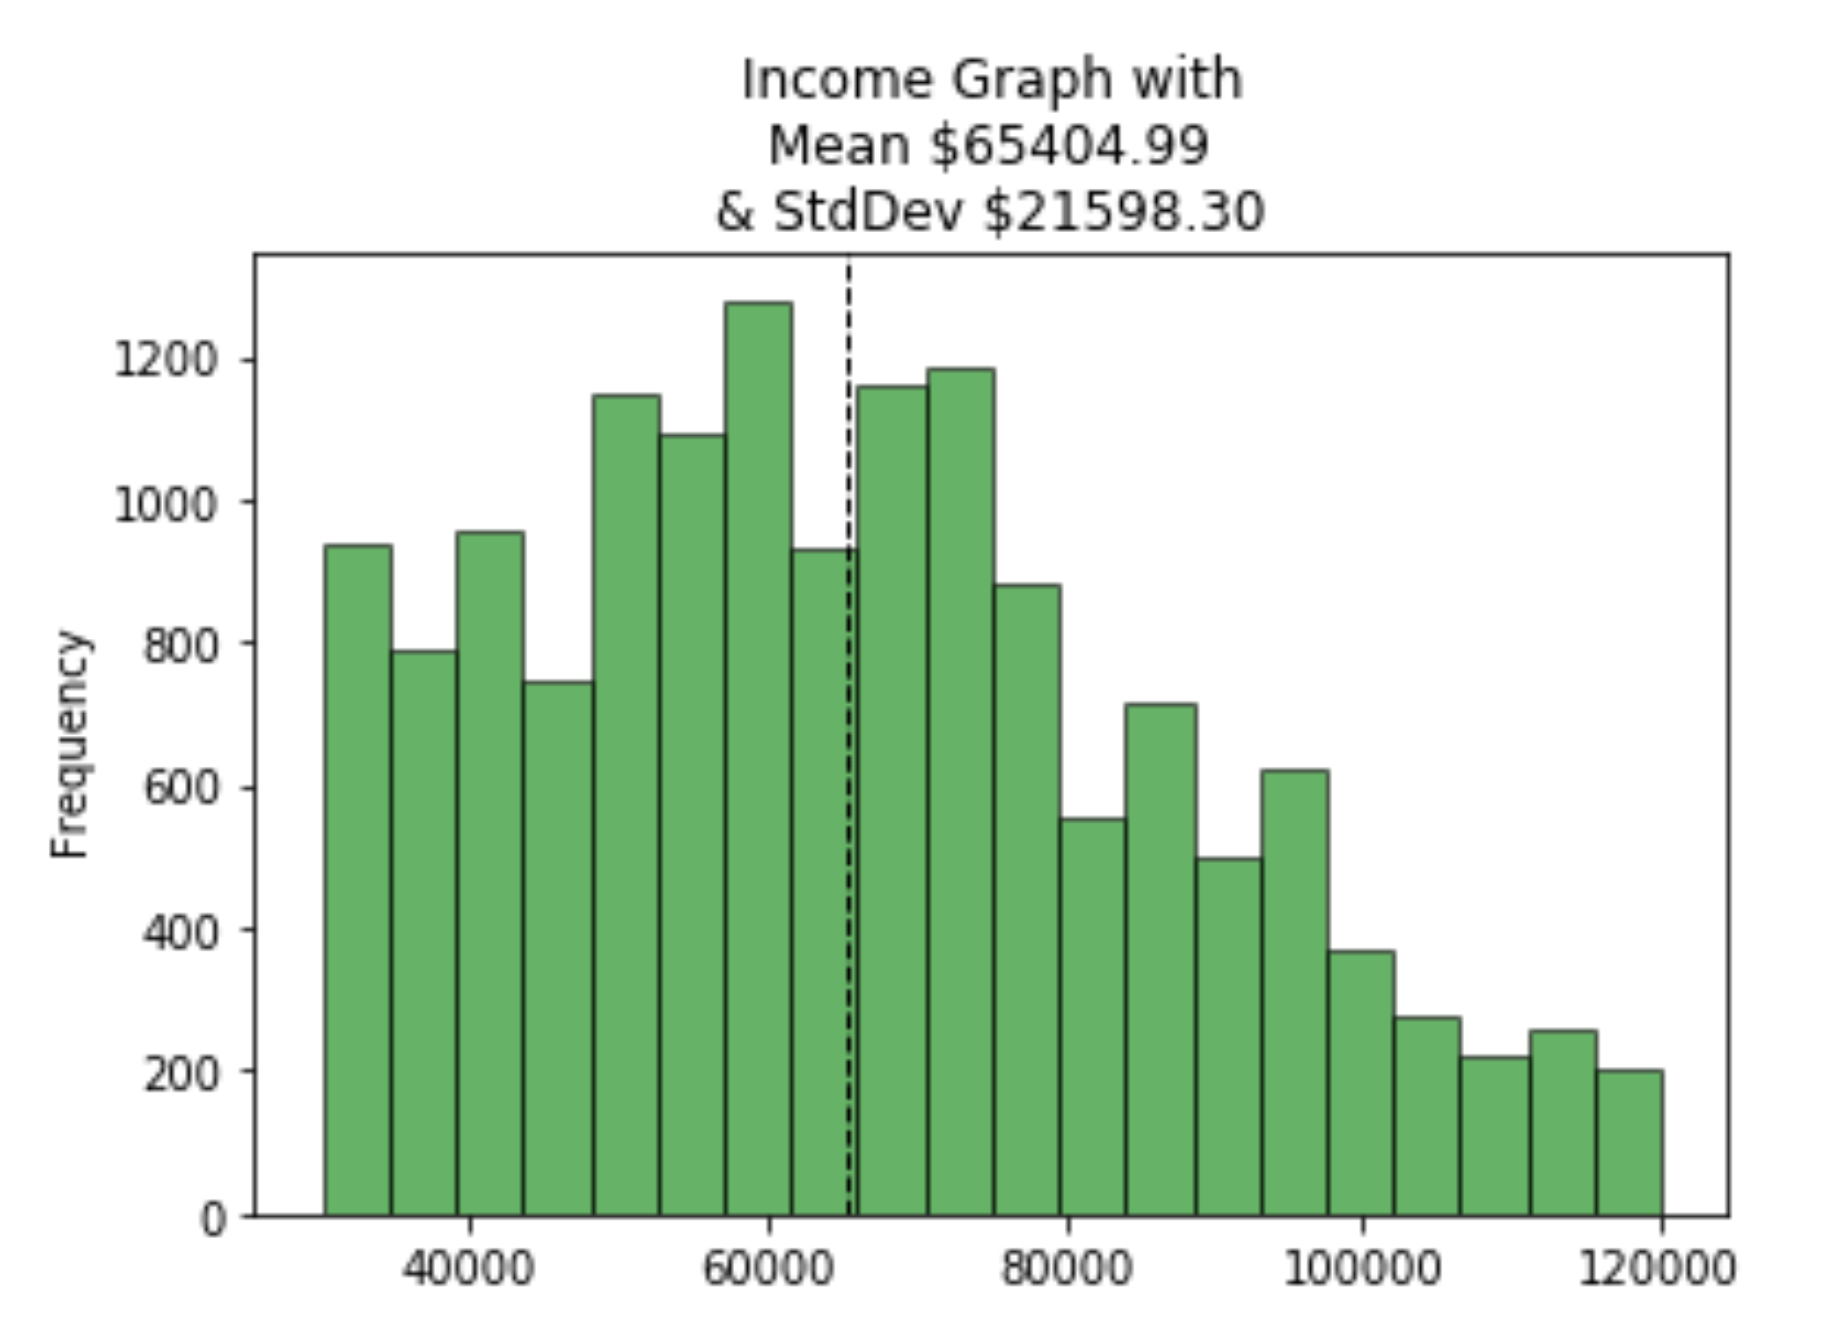
\includegraphics[width=0.9\textwidth, height=7cm]{img/07.png}
    \caption{Profile Income Distribution}
\end{subfigure}

\caption{Profile dataset explorations charts}
\label{fig:g01}
\end{figure}
 
& Transcript dataset exploration
&& This pie chart shows the distribution of events:

\begin{figure}[ht!]
  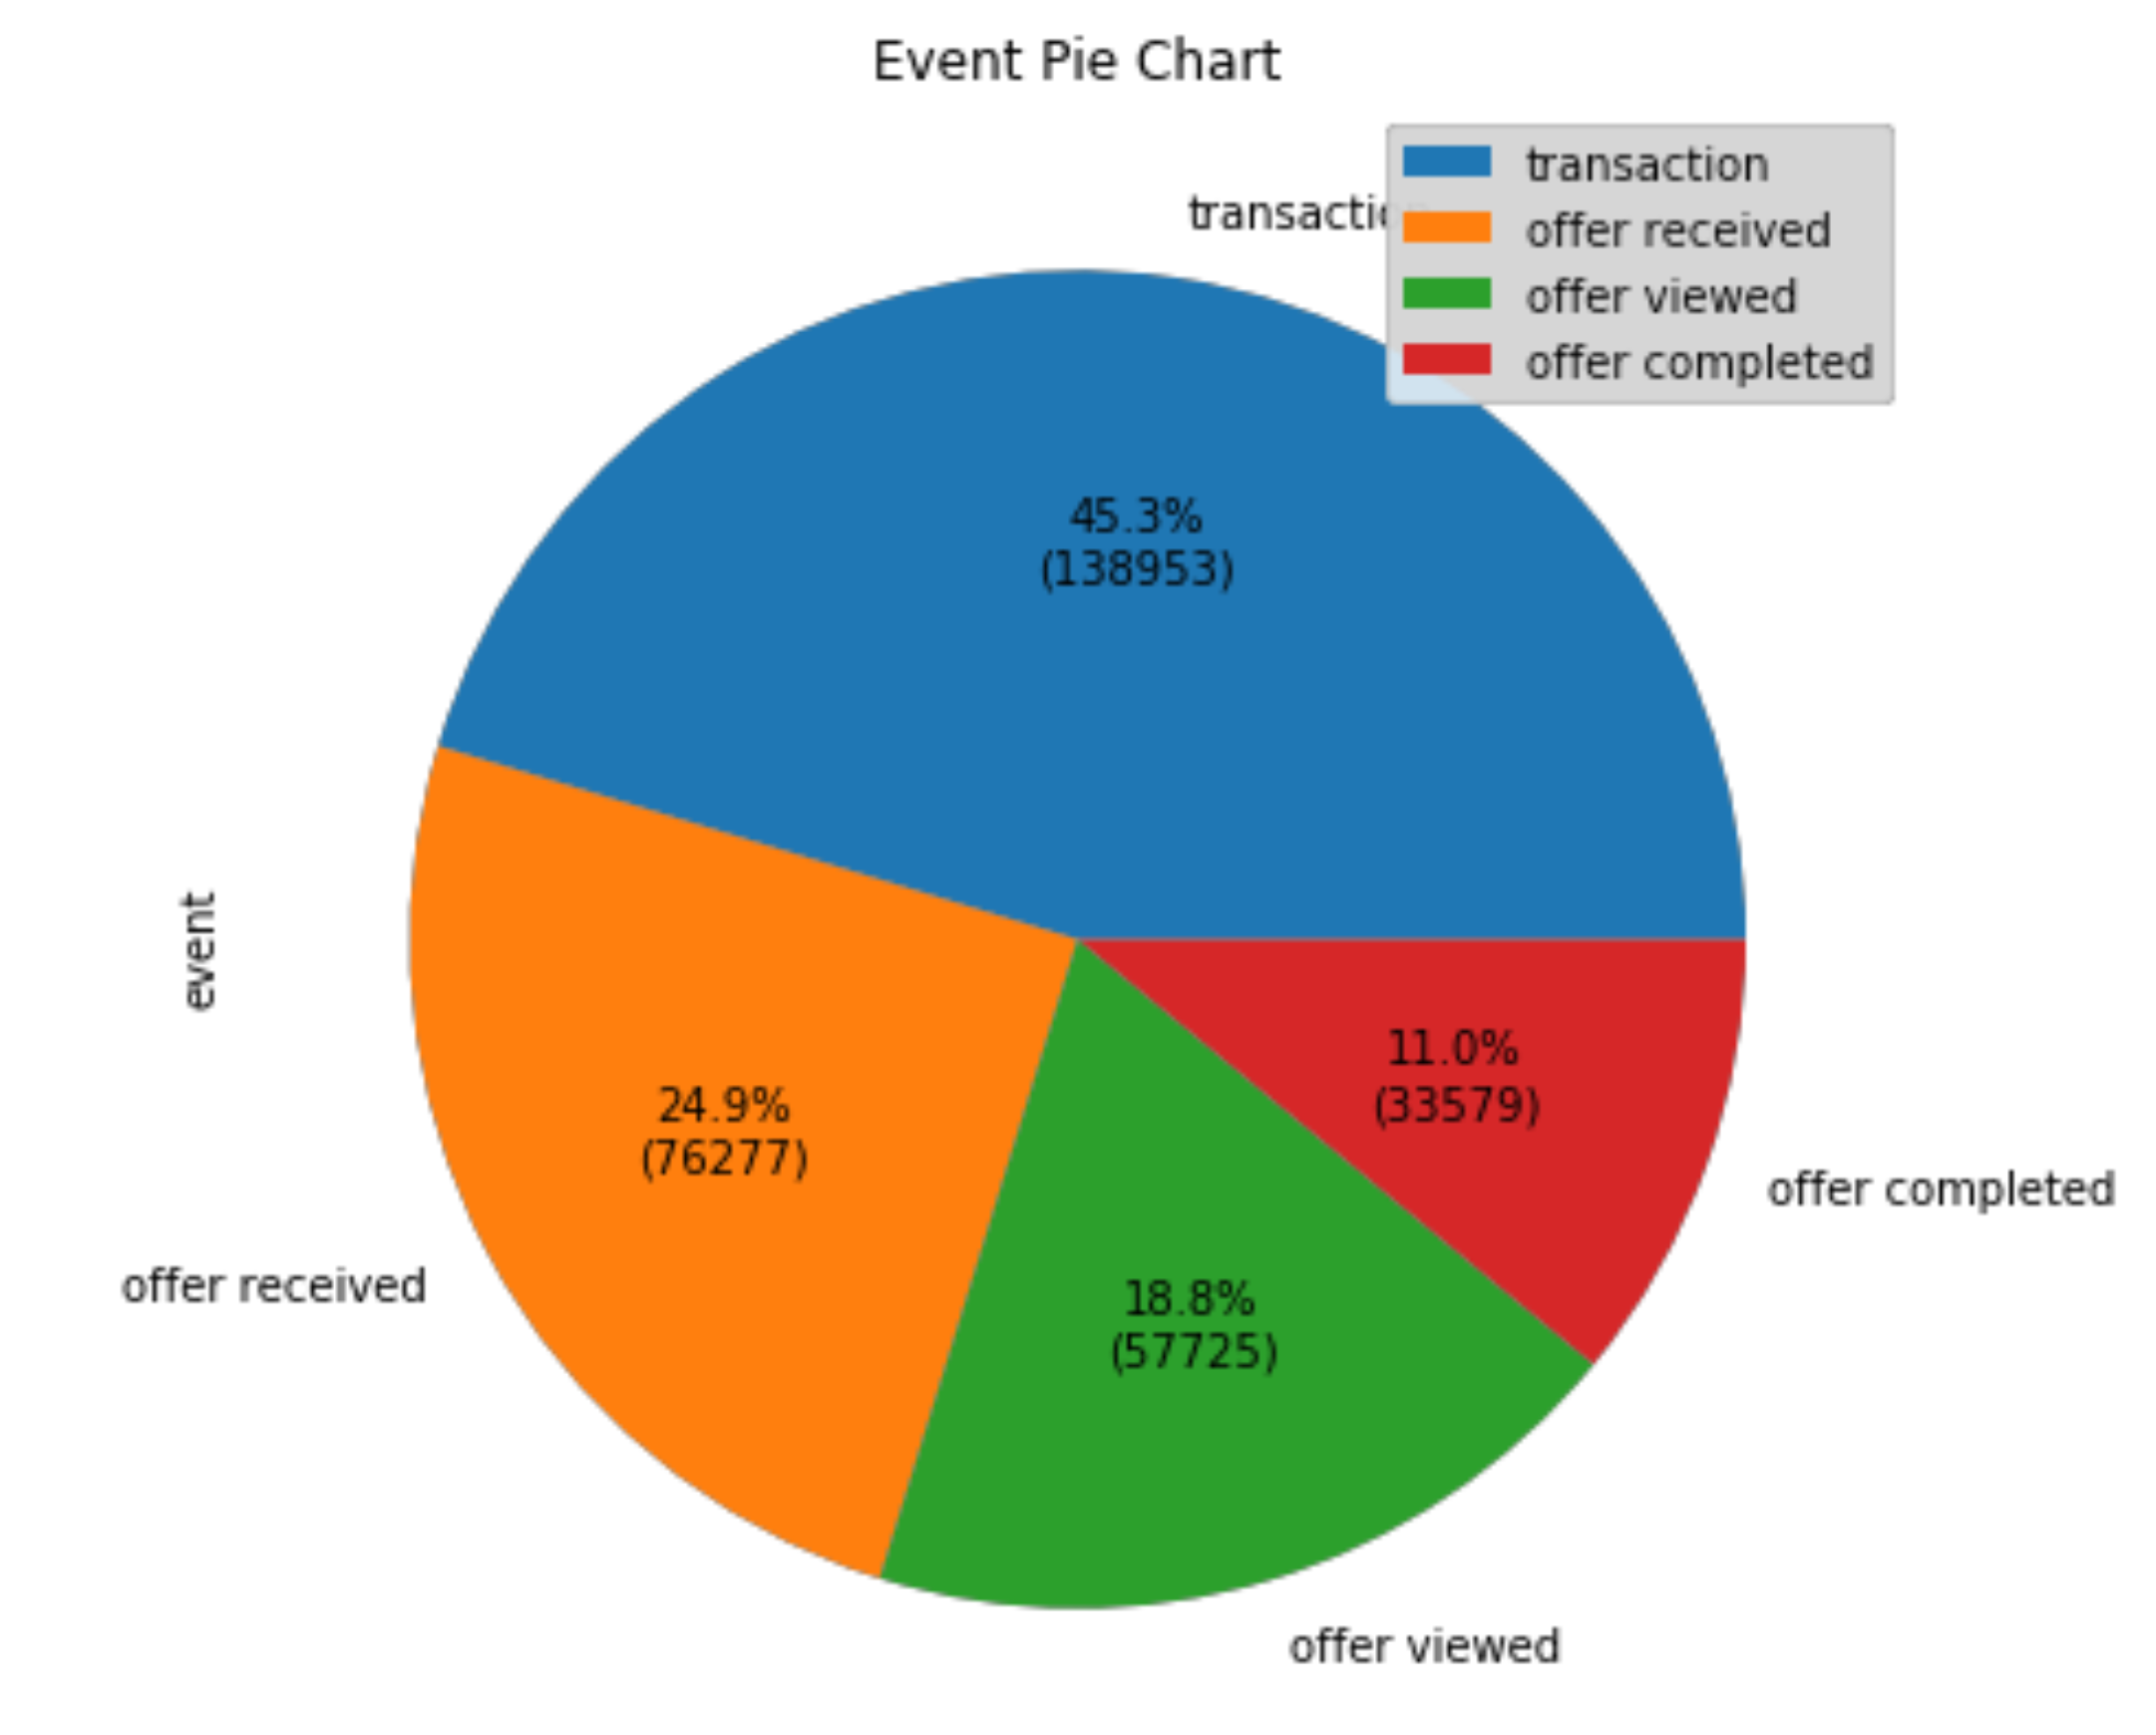
\includegraphics[width=\linewidth]{img/08.png}
  \caption{Transcript Event Percentages and Counts}
  \label{fig:08}
\end{figure}

&& Every customer received at least 1 offer, and some customers received up to 7 offers.
&& Some customers received the same offer multiple times.
&& No customers received multiple offers at the same timestamp.
&& There were many instances where a customer would receive another offer before the previous offer expired, resulting in multiple offers being active at the same time.
\end{easylist}

% ------------------------------------------
\section*{Data preparation}

\subsection*{Joining the Data}
Some of the columns in the Transcript data needed additional feature engineering in order to prepare for building the models. Columns like time, event\_transaction, event\_offer\_received, event\_offer\_viewed, event\_offer\_completed, and trans\_amt needed aggregated into entries per id\_customer and id\_offer. 

My models will focus on customer and offer-related data rather than time or individual event-related data.

I've created a nested dictionary data structure and iterated over the Transcript data capturing the following for each id\_customer:\newline
\begin{easylist}
&& For each offer received: the ‘num\_times\_received’, the ‘num\_times\_viewed’, the ‘num\_times\_completed’, and ‘total\_amt\_spent\_towards\_offer’.
&& Also the ‘total\_amt\_spent\_not\_in\_offer’ to capture all money spent when no offers were active.\newline
\end{easylist}
 
This resulted in the following columns added to the data for additional analysis:\newline

\begin{easylist}
&& ‘amount\_spent\_not\_in\_offer’ 
&& ‘num\_times\_received’
&& ‘num\_times\_viewed’
&& ‘num\_times\_completed’
&& ‘total\_amt\_spent\_towards\_offer’
&& ‘avg\_amt\_spent\_towards\_offer’\newline
\end{easylist}
 
After creating these new columns, I could safely remove the time, event\_transaction, event\_offer\_received, event\_offer\_viewed, event\_offer\_completed, and trans\_amt columns from Transcript.

I then merged the Transcript, Portfolio, and Profile data into a Combined dataframe.

\begin{figure}[ht!]
  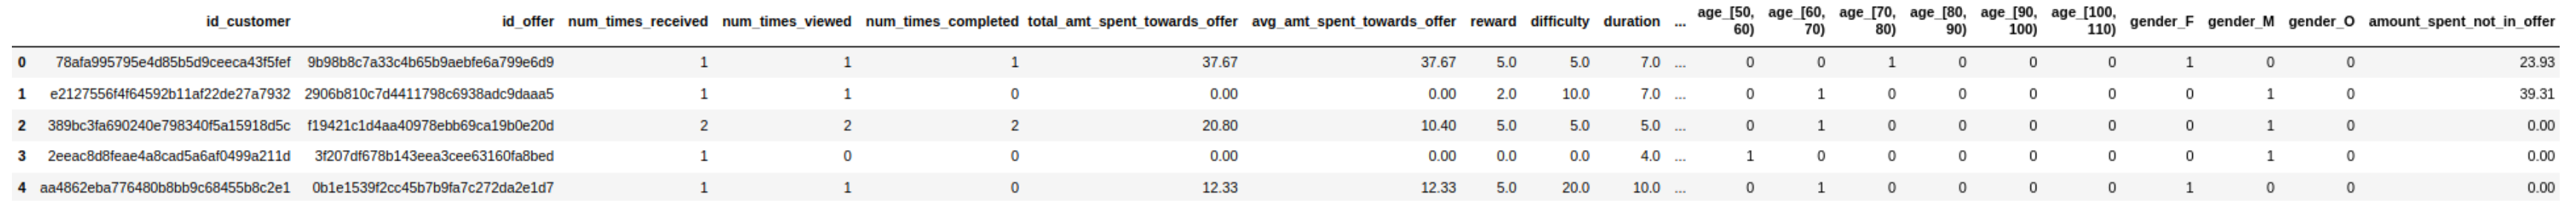
\includegraphics[width=\linewidth, height=1.5cm]{img/09.png}
  \caption{The Combined Dataframe after merging Transcript, Portfolio, and Profile}
  \label{fig:09}
\end{figure}


\subsection*{Preparing the Data for the Models}
At this point, all of our data is based on each id\_customer / id\_offer pair. In order for the data to be ready for the models, I added/removed the following columns:\newline

\begin{easylist}
&& Added a column to indicate if the specific offer was “successful” or not. An offer is “successful” if the customer completed it at least once.
&& Removed all “Informational” rows, since they are never completed.
&& Removed rows where id\_offer is NaN. These occur when a
transaction event occurs outside of an offer.
&& Removed the id\_customer column, since we want the models to generalize to look at the offer as a whole.
&& Removed the num\_times\_received, num\_times\_viewed, num\_times\_completed, membership\_year, and amount\_spent\_not\_in\_offer as these were only used for creating graphs.
&& Removed the email column, since every offer is sent via email.
&& Removed avg\_amt\_spent\_towards\_offer and total\_amt\_spent\_towards\_offer since we only care that they completed the offer at least once.\newline
\end{easylist}

My final Combined column list is:
\begin{figure}[ht!]
  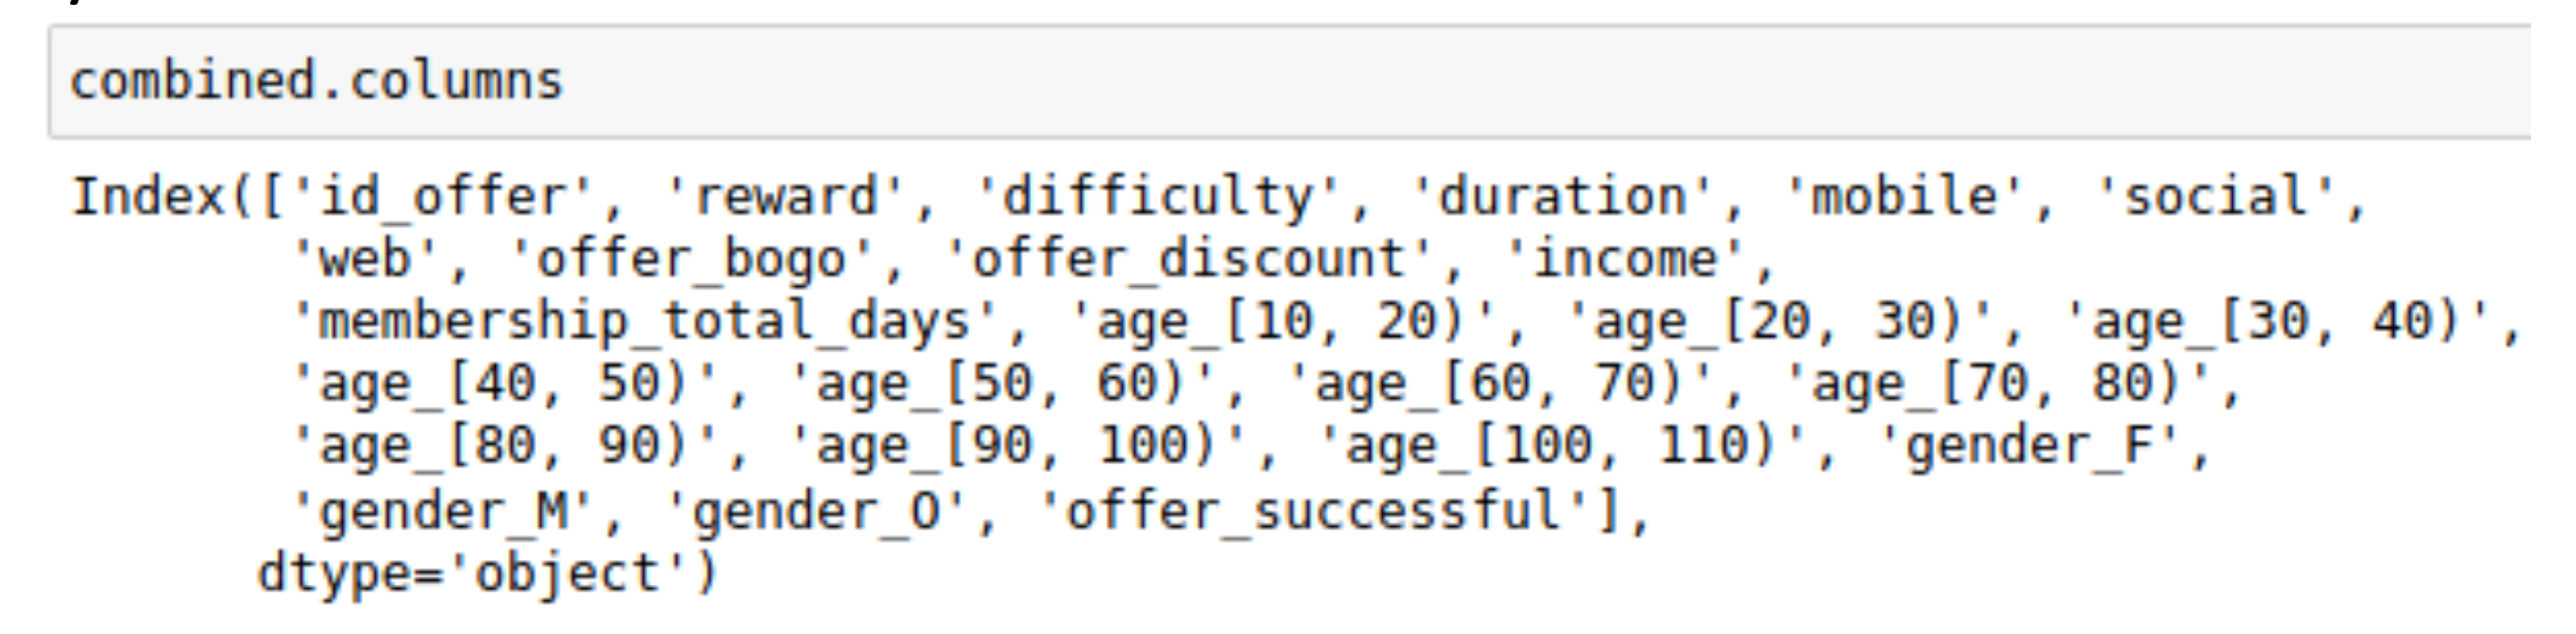
\includegraphics[width=\linewidth]{img/10.png}
  \caption{List of Columns in my Final Combined Dataframe}
  \label{fig:10}
\end{figure}
 
An important data preparation step is scaling the data to be between 0 and 1. This is to prevent the model from incorrectly assigning importance to one column with extremely large values (such as income in the tens of thousands) over another column with much smaller values (such as duration which is 10 days or less).

To scale the data between 0 and 1, I used Scikit Learn’s MinMaxScaler. I scaled the reward, difficulty, duration, and income columns in my Combined dataset.

Then I created my Training/Testing/Validation datasets with a 60/20/20 split.

% --------------------------------------------
\section*{Evaluation metrics}

False negatives are the worst kind of error we can make for this project. If we produce a False Positive, the user will likely just ignore our marketing effort and result in possibly some wasted effort on our part. In extreme cases, the user could view False Positives as harassment and be turned off by our brand. Because of this extreme case, False Positives are still important but not as important as False Negatives.

False Negatives result in a missed opportunity to market to a receptive customer. This can result in the business not making sales that they would have otherwise made.

Precision is used when the cost of False Positives is high. Recall is used when the cost of False Negatives is high. In our case we want to consider the cost of both but focus more on False Negatives. To do this we can use the F2 score, which puts more emphasis on recall.

The F2 score is defined as:
\begin{equation}
	F_2 = (1+2^2) \cdot \dfrac{precision \cdot recall}{(2^2 \cdot precision)+recall}
\end{equation}
\newpage

% ----------------------------------
\section*{Model training}

\subsection*{Benchmark model - logistic regression model}

I used Scikit Learn’s Logistic Regression model. I originally started with the default values (only setting random\_state to get the same results every time), but found that the default max iterations value of 100 was too low. I increased the max iterations to 1000 and got better results.

 The accuracy is 0.71208, F1 Score is 0.79208, F2 Score is 0.83016, and confusion matrix is:
 
\begin{figure}[ht!]
  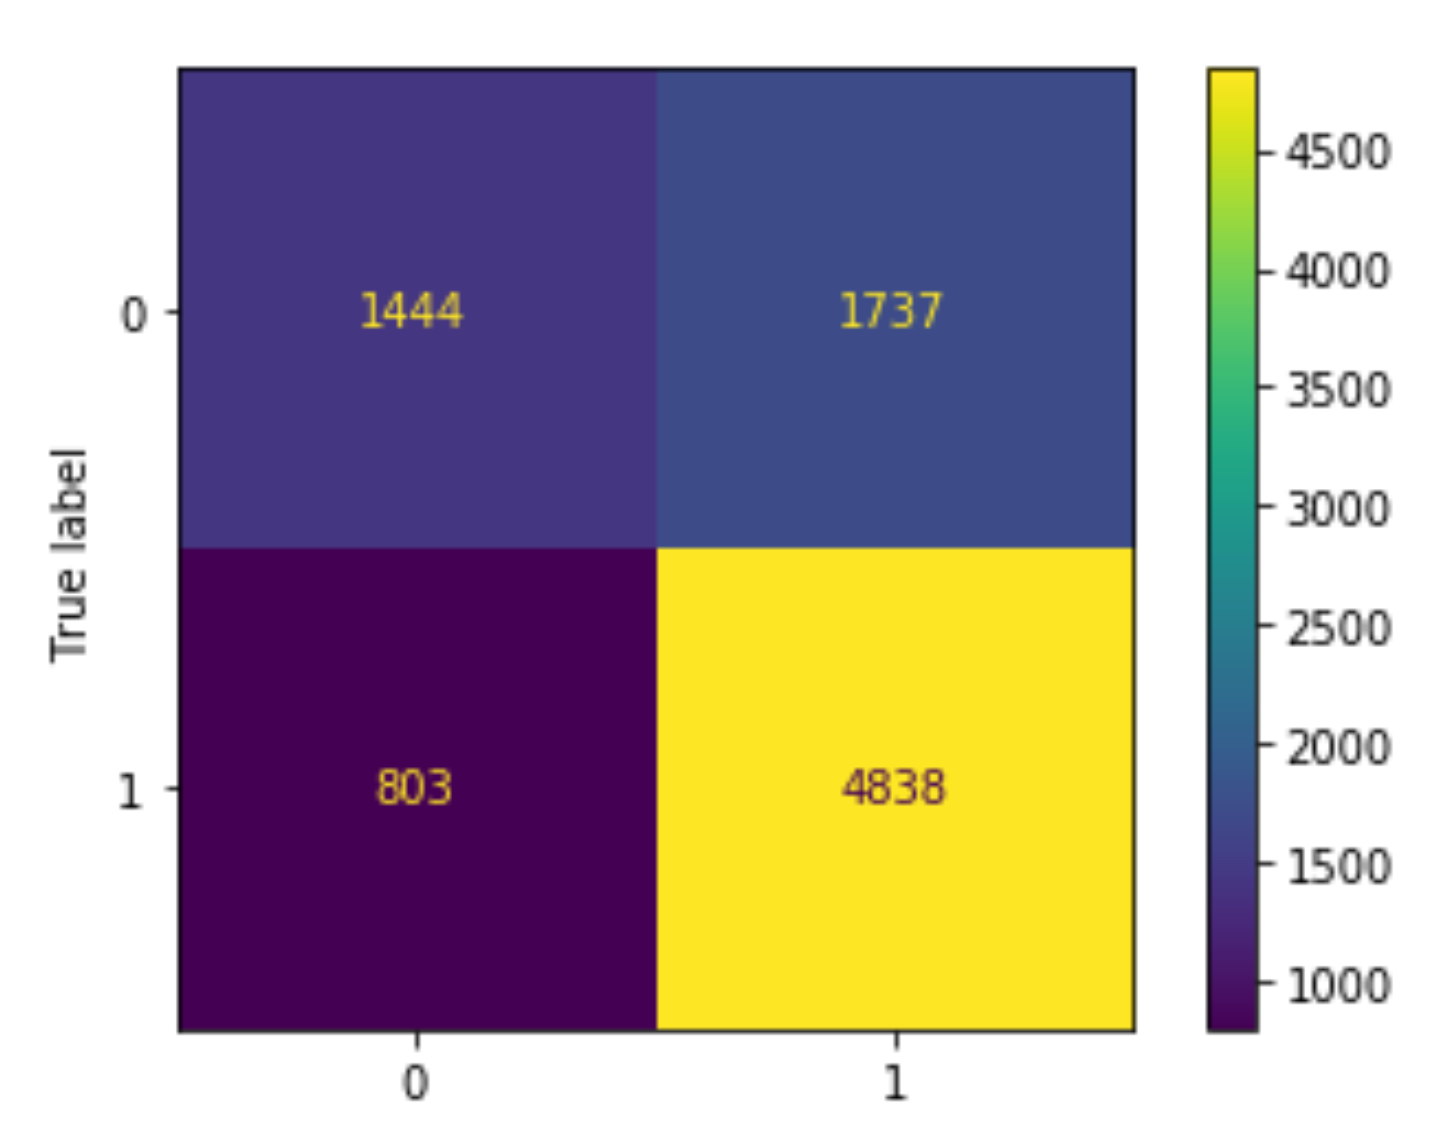
\includegraphics[width=0.5\linewidth]{img/11.png}
  \centering
  \caption{Logistic Regression Confusion Matrix}
  \label{fig:11}
\end{figure}

\subsection*{Support Vector Machine (SVM)}
 I used Scikit Learn’s SVM SVC implementation which is a C-Support Vector Classifier. C is a regularization parameter where the strength of regularization is inversely proportional to C (with C > 0). Gamma is the kernel coefficient for the Radial Basis Function (RBF) kernel.
  
After Hyperparameter Tuning (described in detail in the below section) I settled on C=10,000 and gamma=1e-05.

The accuracy is 0.72463, F1 Score is 0.78873, F2 Score is 0.80353, and confusion matrix is:

\begin{figure}[ht!]
  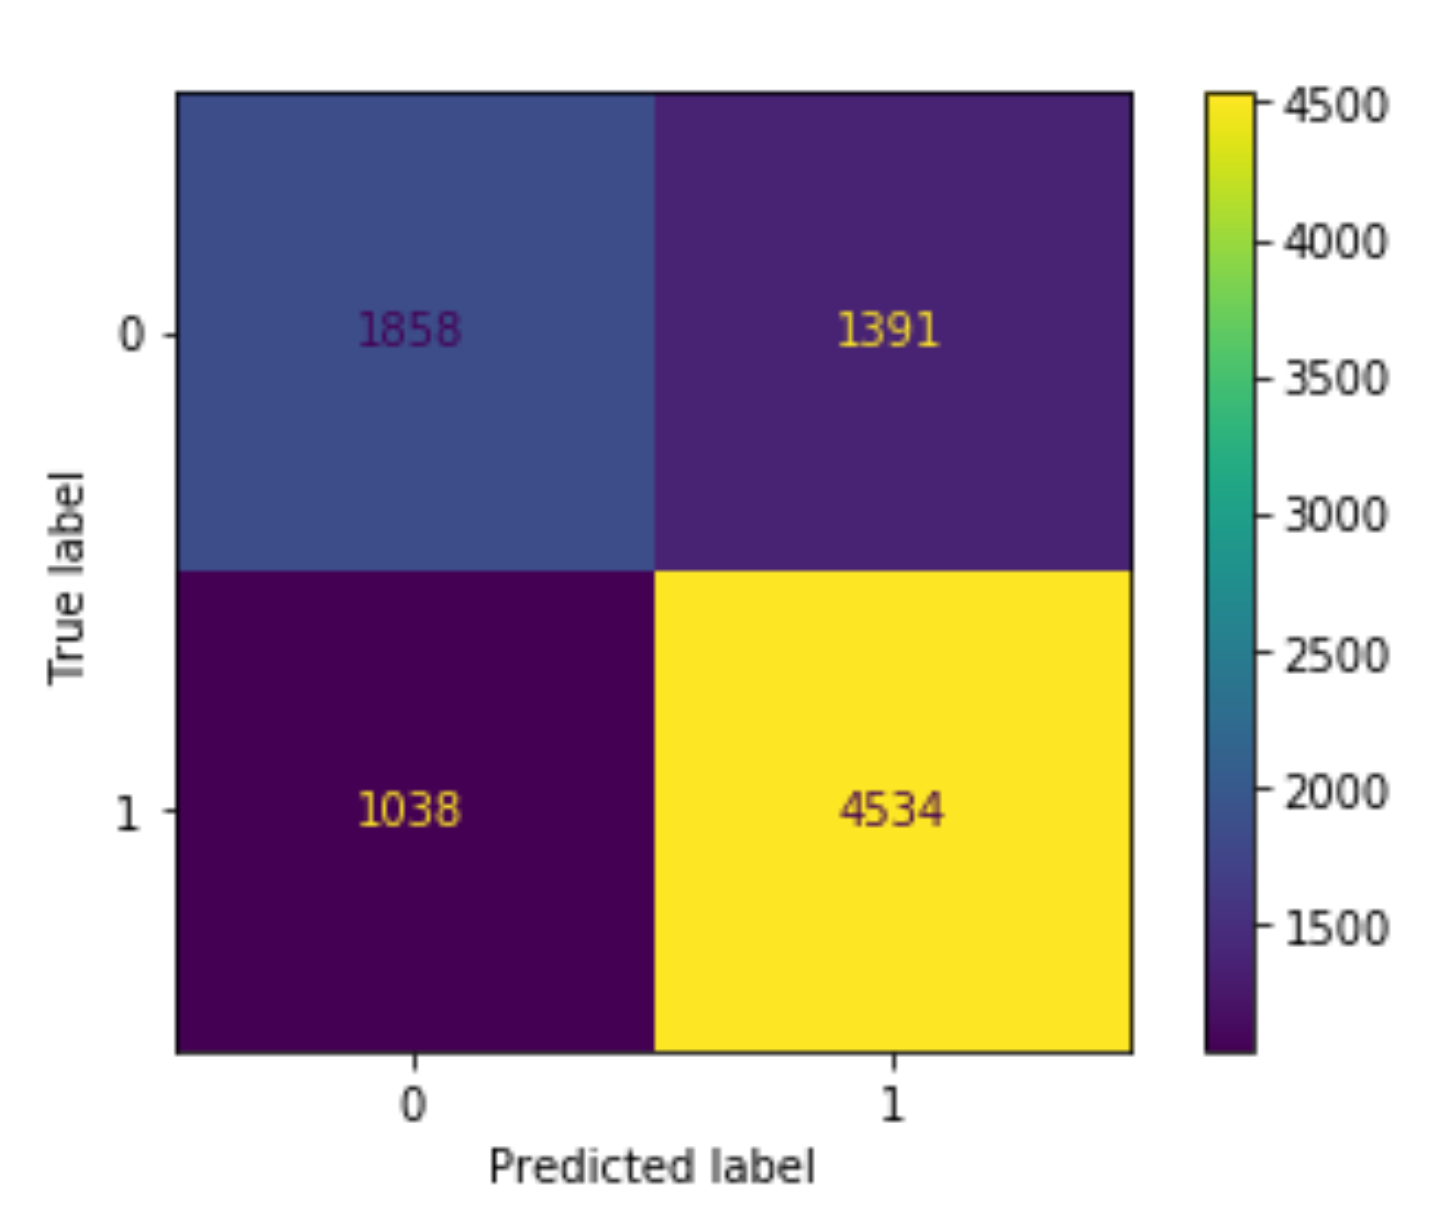
\includegraphics[width=0.5\linewidth]{img/12.png}
  \centering
  \caption{SVM Confusion Matrix}
  \label{fig:12}
\end{figure}

\subsection*{Neural Network model} 
 I used the TensorFlow 2.0 framework for building and training my model.
 I will discuss the Hyperparameter Tuning in-depth in the next section. The hyperparameters selected are:\newline
 
\begin{easylist}
&& 2 Hidden Layers
&& Hidden Layer 1 has 128 nodes, with ReLU activation functions, and Dropout value of 0.3
&& Hidden Layer 2 has 32 nodes, with ReLU activation functions, and Dropout value of 0.2
&& I used the Adam optimizer with a learning rate of 1e-4
&& My loss metric was Binary Cross Entropy
&& I used an Early Stopping callback monitoring the validation loss. This stopped the training if the validation loss had not decreased within 20 epochs.
&& Since I had the Early Stopping callback, I set the number of epochs equal to the number of training data rows (26,463). Because of the Early Stopping, I never exceeded 400 epochs.
&& I also used a Model Checkpoint that saved the best model based on the minimum validation loss found.\newline
\end{easylist}

\begin{figure}[ht!]
  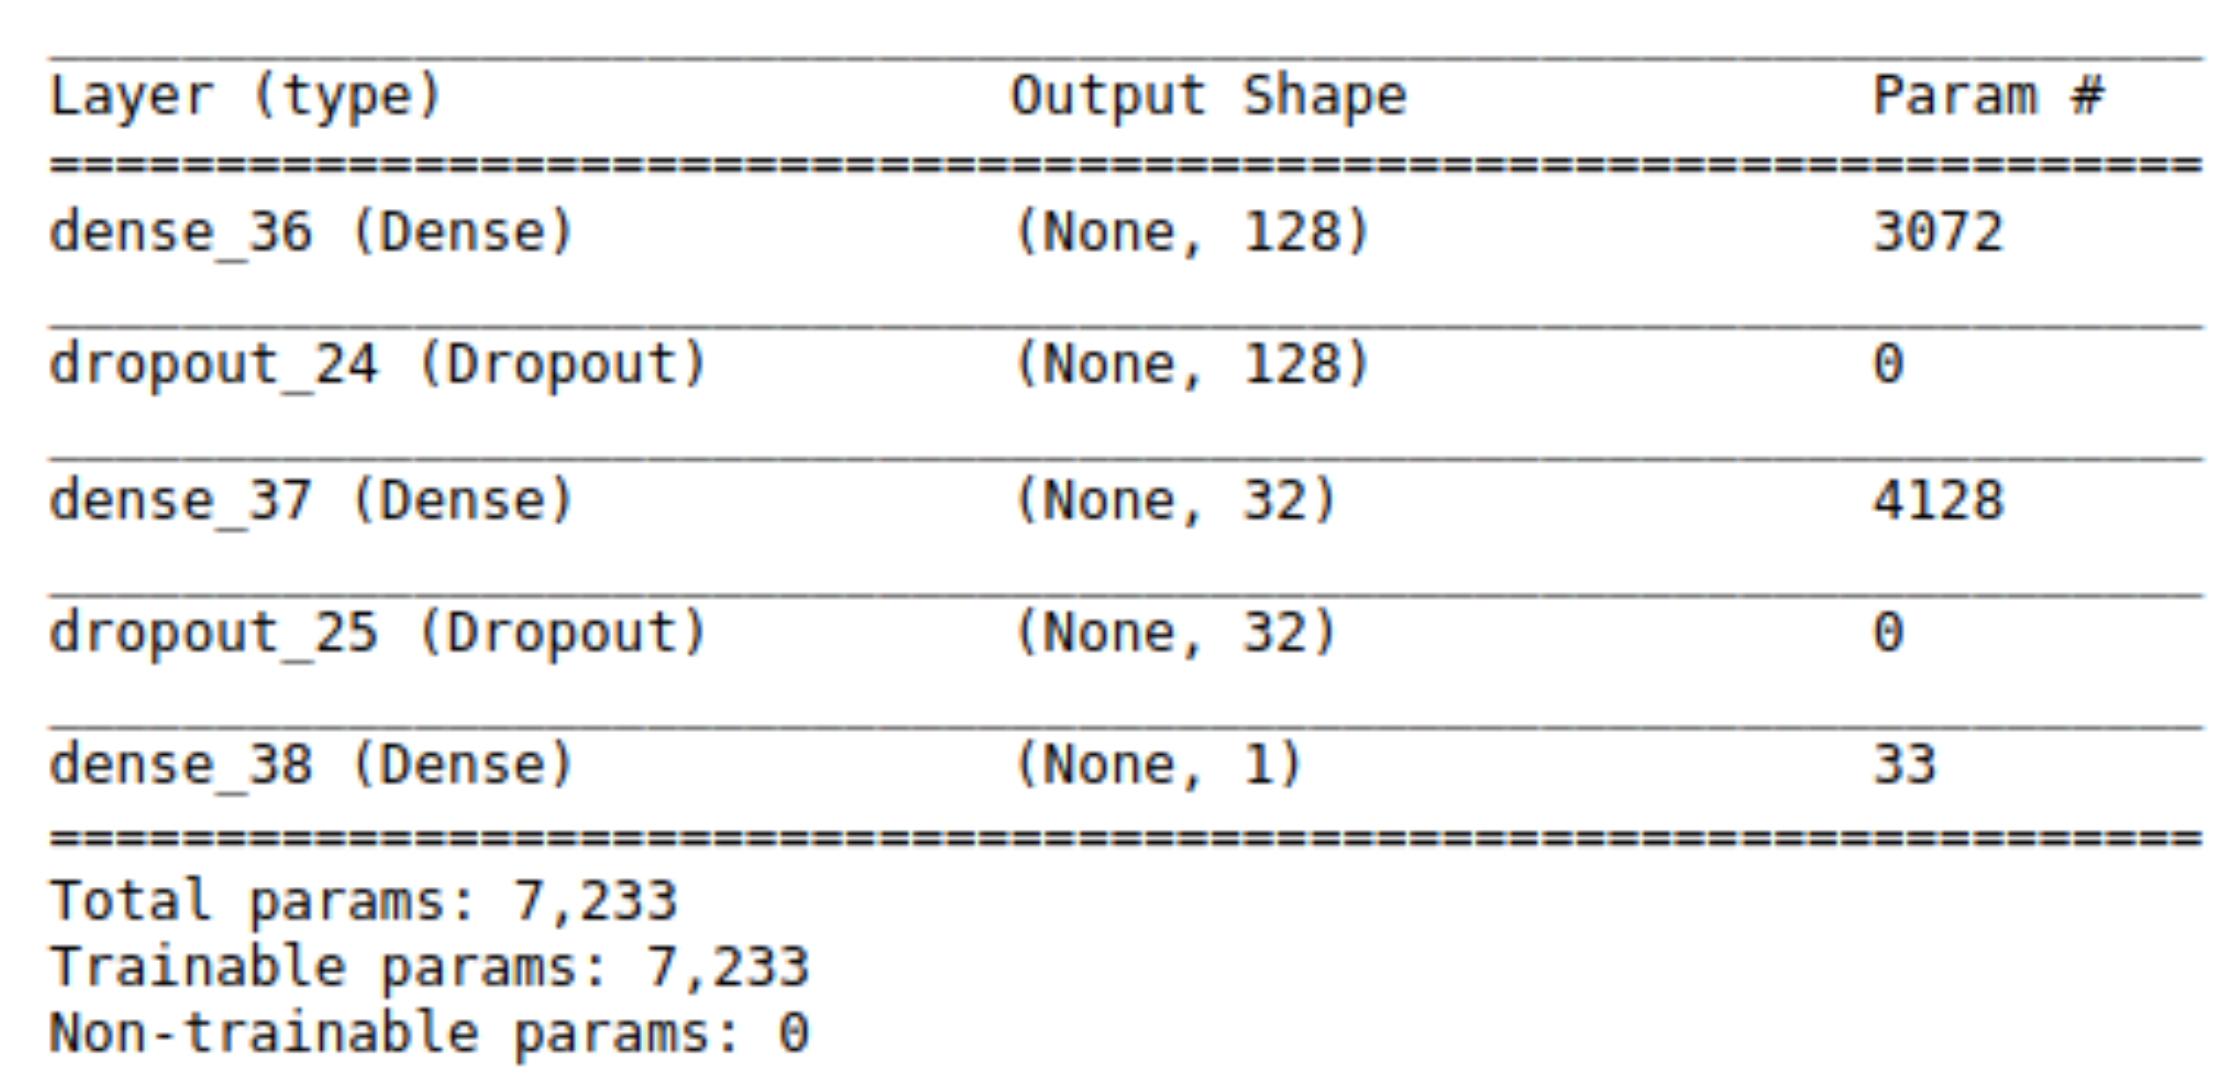
\includegraphics[width=0.7\linewidth]{img/13.png}
  \centering
  \caption{TensorFlow 2.0 Keras Model Summary}
  \label{fig:13}
\end{figure}

The accuracy is 0.71163, F1 Score is 0.79726, F2 Score is 0.84863, and confusion matrix is:

\begin{figure}[ht!]
  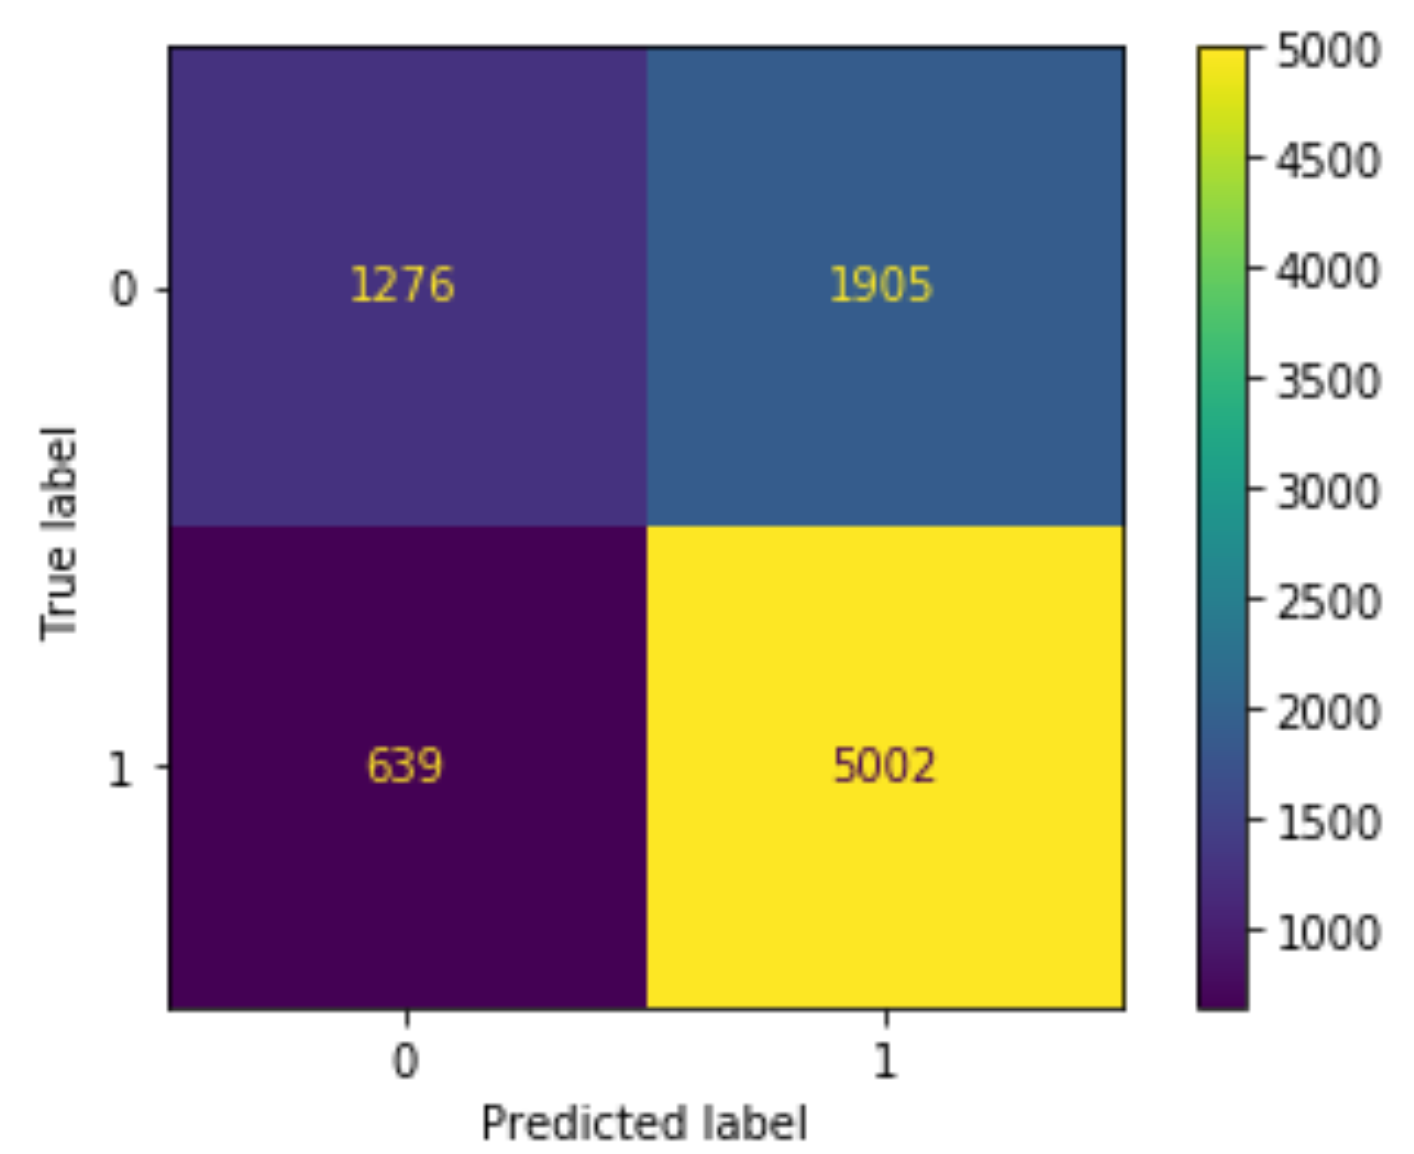
\includegraphics[width=0.5\linewidth]{img/14.png}
  \centering
  \caption{Neural Network Confusion Matrix}
  \label{fig:14}
\end{figure}

\newpage
\subsection*{Comparing the Models}
Below is a graph showing the metrics for each model against the Test Set:

\begin{figure}[ht!]
  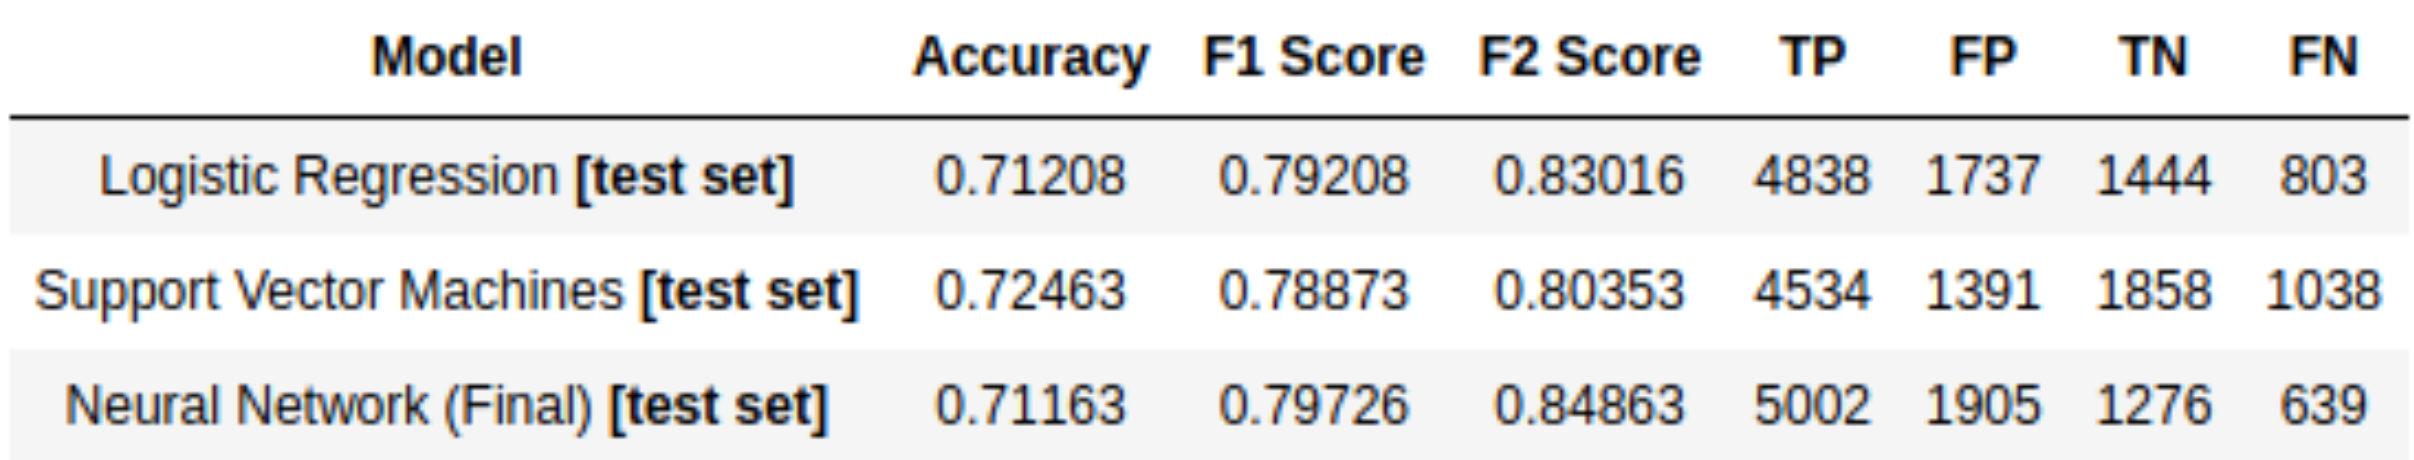
\includegraphics[width=0.9\linewidth]{img/15.png}
  \centering
  \caption{Final Metrics using the Test Set}
  \label{fig:15}
\end{figure}

The Neural Network performed the best out of the 3 models with an F2 Score of 0.84863 and with the lowest False Negative count of 639. It also has the most True Positives. As stated previously, the False Negatives is the worst kind of error for us since it is a missed opportunity to market to a receptive customer.

The Logistic Regression (baseline model) was a close second to the Neural Network.

The Support Vector Machine performed the worst overall out of the 3 models.

% ---------------------------------
\section*{Hyperparameter tuning}

\subsection*{SVM Tuning}
For determining the C and gamma values for the SVM SVC model, I got my idea
from here. I used grid search to look for 10 ‘C’ values in log space between 10−2 and 104, and 10 gamma values in log space between 10−9 and 103. The best parameters found were C of 10,000 and gamma of 1e-05 which received an accuracy score of 0.73 on the validation set.

\subsection*{Neural Network (NN) Tuning}
For determining hyperparameters for the NN I used TensorFlow’s TensorBoard and the HParams Dashboard. One issue I encountered was my Jupyter Notebook kernel repeatedly crashed when trying to perform hyperparameter tuning for the neural network. I eventually wrote a separate Python program do the hyperparameter tuning.

I went through 4 iterations when finding the NN hyperparameters, each time narrowing the focus.

The first iteration tested the following:\newline
\begin{easylist}
&& Hidden Layer 1 Number of Nodes: 32, 64, 128, 256
&& Hidden Layer 1 Dropout: 0.1, 0.2, 0.3, 0.4, 0.5
&& Number of Hidden Layers: 1 or 2
&& Hidden Layer 2 Number of Nodes: 32, 64, 128, 256
&& Hidden Layer 2 Dropout: 0.1, 0.2, 0.3, 0.4, 0.5
&& Optimizer: Adam or SGD
&& Learning Rate: 1e-5, 1e-4, 1e-3 \newline
\end{easylist}

This iteration eventually ran out of memory before fully completing, but it gave me enough of an idea to move onto other iterations. I knew from this first iteration that Adam received better results than SGD, so I removed SGD from later iterations.

The second iteration used 1 Hidden Layer and tested the following:\newline
\begin{easylist}
&& Hidden Layer 1 Number of Nodes: 32, 64, 128
&& Hidden Layer 1 Dropout: 0.1, 0.2, 0.3, 0.4, 0.5
&& Number of Hidden Layers: 1
&& Optimizer: Adam
&& Learning Rate: 1e-4, 1e-3 \newline
\end{easylist}

The third iteration used 2 Hidden Layers and tested the following:\newline
\begin{easylist}
&& Hidden Layer 1 Number of Nodes: 32, 64, 128
&& Hidden Layer 1 Dropout: 0.1, 0.2, 0.3, 0.4, 0.5
&& Number of Hidden Layers: 2
&& Hidden Layer 2 Number of Nodes: 32, 64, 128
&& Hidden Layer 2 Dropout: 0.1, 0.2, 0.3, 0.4, 0.5
&& Optimizer: Adam
&& Learning Rate: 1e-4, 1e-3
\end{easylist}

From this I was able to determine 2 Hidden Layers was better than 1, and smaller learning rate was better. I also found that 128 nodes in Hidden Layer 1 and 32 nodes in Hidden Layer 2 resulted in the best results.

The fourth iteration further refined the previous iterations and tested the following:\newline
\begin{easylist}
&& Hidden Layer 1 Number of Nodes: 128
&& Hidden Layer 1 Dropout: 0.1, 0.2, 0.3
&& Number of Hidden Layers: 2
&& Hidden Layer 2 Number of Nodes: 32
&& Hidden Layer 2 Dropout: 0.1, 0.2, 0.3
&& Optimizer: Adam
&& Learning Rate: 7.5e-5, 8.75e-5, 1e-4\newline
\end{easylist}

Below is a table showing the best results from each iteration:

\begin{figure}[ht!]
  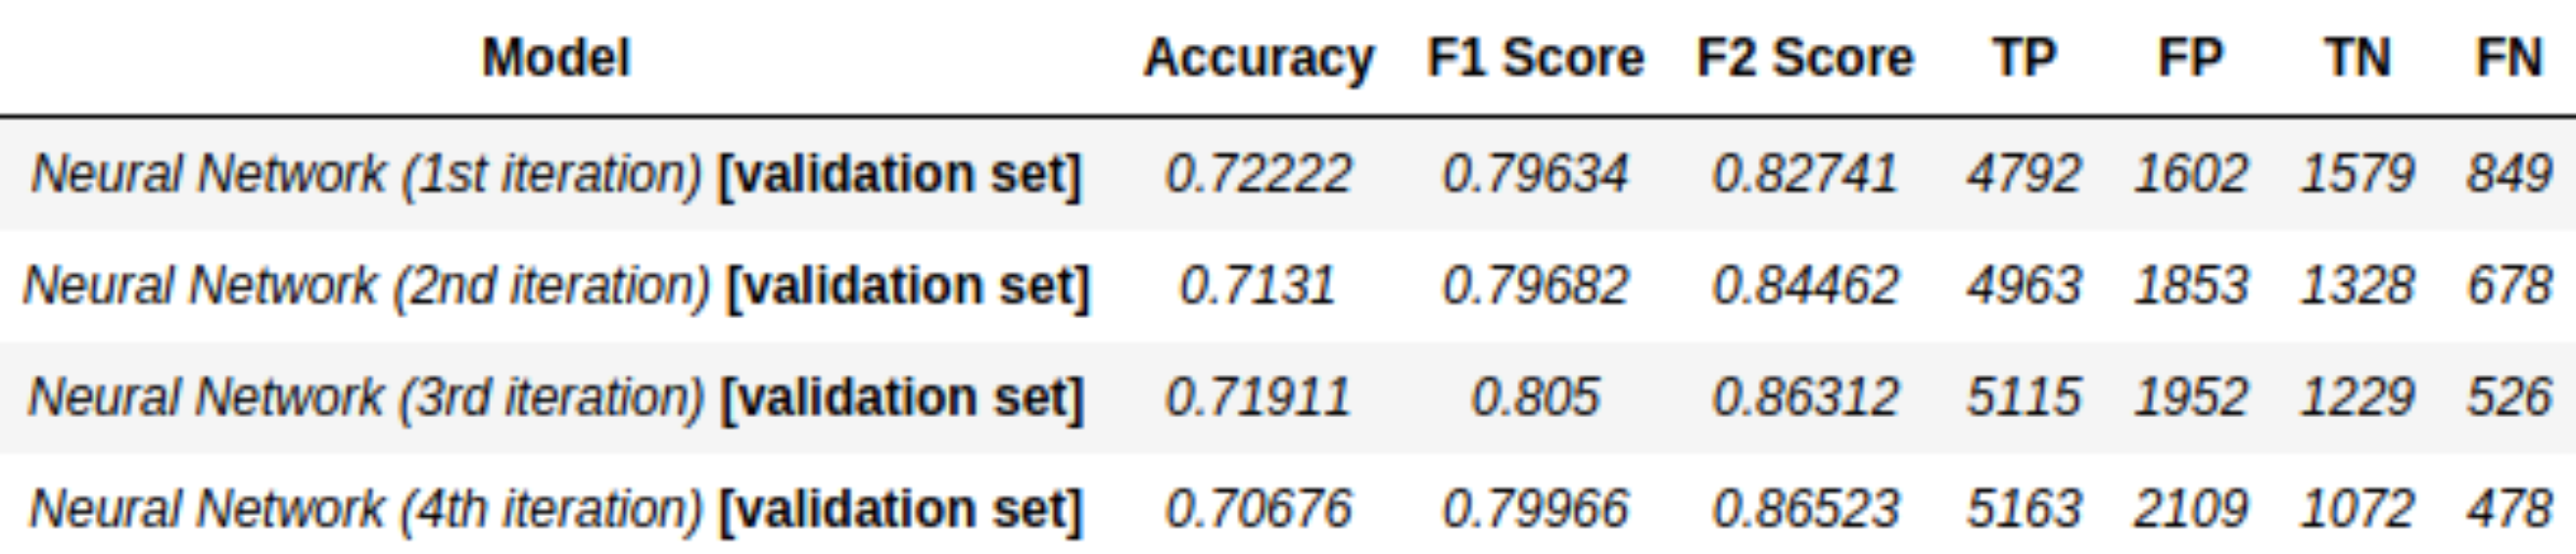
\includegraphics[width=0.9\linewidth]{img/16.png}
  \centering
  \caption{Hyperparameter Tuning Scores for each Iteration against Validation Set}
  \label{fig:16}
\end{figure}

The best parameters from the fourth iteration were the final parameters used.\newline
\begin{easylist}
&& Hidden Layer 1 Number of Nodes: 128
&& Hidden Layer 1 Dropout: 0.3
&& Number of Hidden Layers: 2
&& Hidden Layer 2 Number of Nodes: 32
&& Hidden Layer 2 Dropout: 0.2
&& Optimizer: Adam
&& Learning Rate: 1e-4\newline
\end{easylist}

Below is a screenshot from the Tensorboard HParams Dashboard showing the best hyperparameters from the final iteration highlighted in green. The blue line has a higher F2 Score but also classifies all data as Positive (send offer), TP or FP, and does not classify any as Negative (don’t send offer), TN or FN. The colors range from bright red for highest accuracy to dark blue for lowest accuracy. The line in green is the one I selected.

\begin{figure}[ht!]
  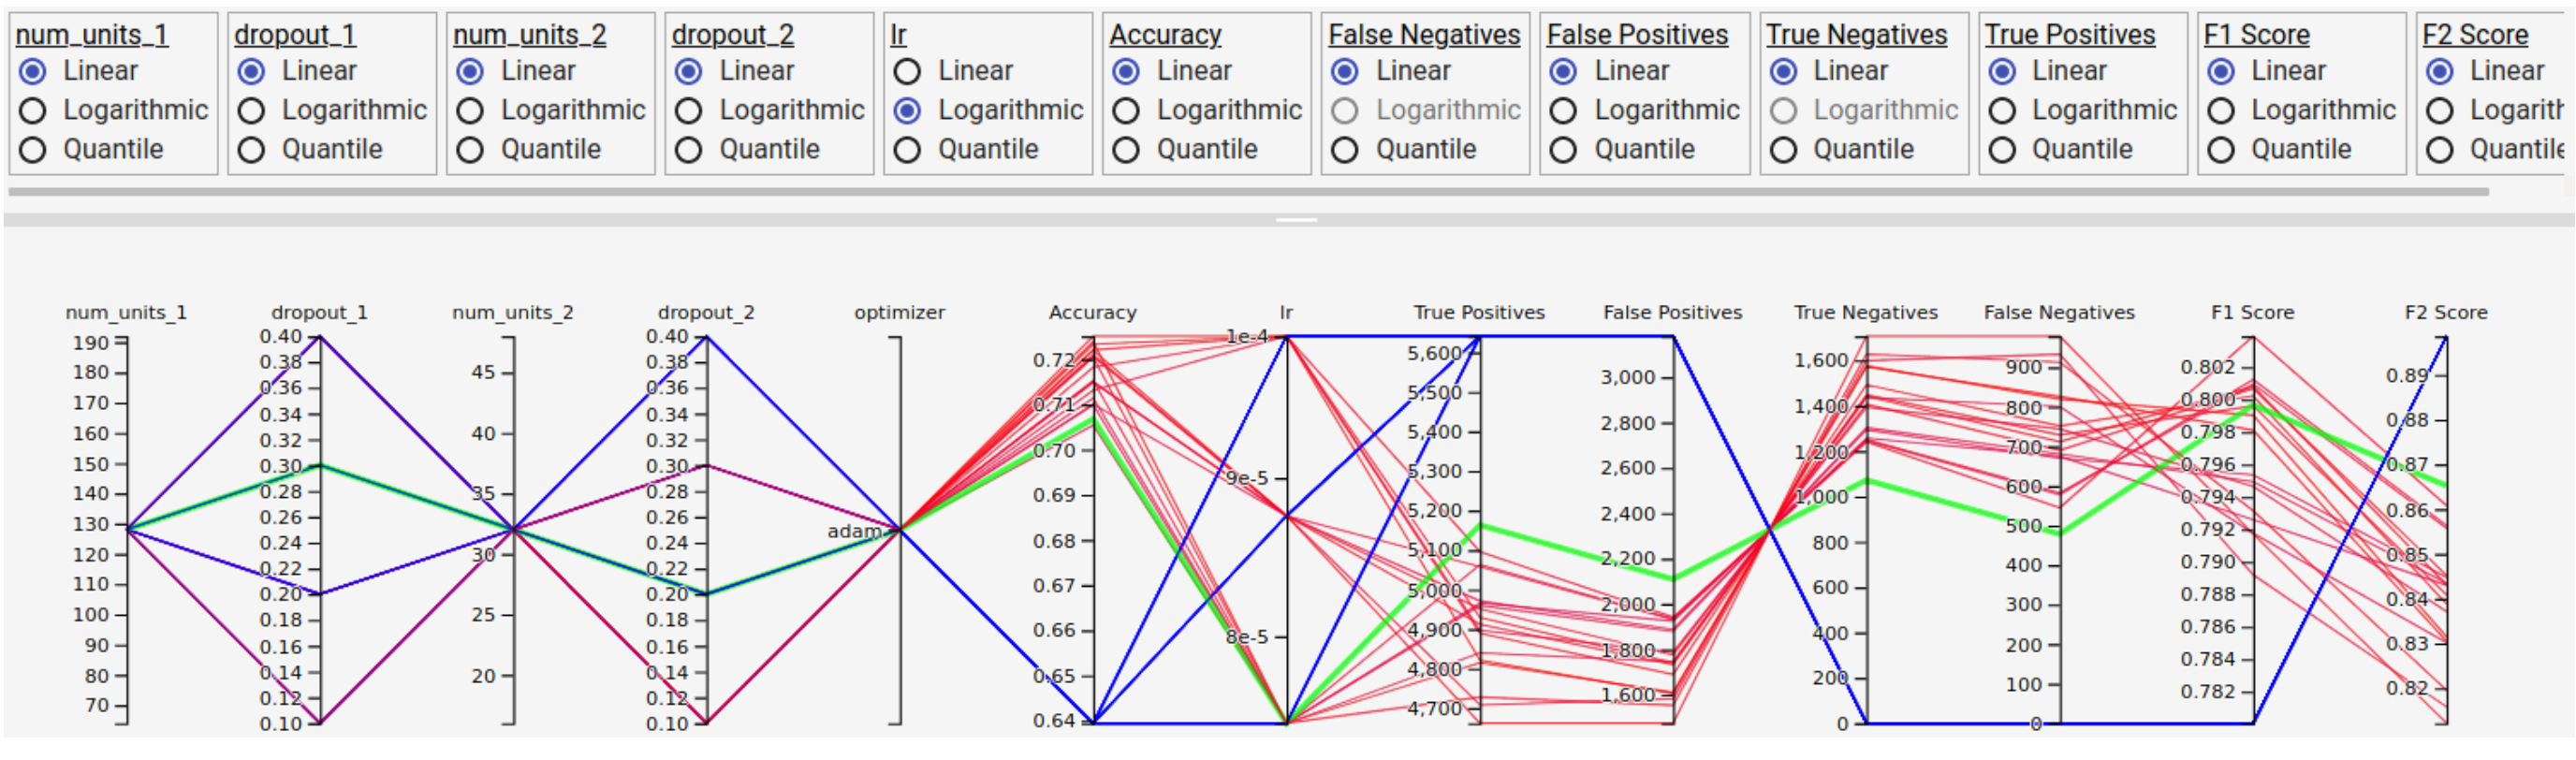
\includegraphics[width=0.9\linewidth]{img/17.png}
  \centering
  \caption{Params Dashboard from Final Iteration (Best Hyperparameters in Green)}
  \label{fig:17}
\end{figure}
 
% --------------------------------
\newpage
\section*{Conclusion}
For this project I have analyzed, cleaned, performed feature engineering, and created 3 models using the Starbucks data. I have created a Neural Network model that successfully performs propensity modeling with an F2 Score of 0.84863 on the Test Set and the lowest False Negative score out of all my models. As mentioned previously, Starbucks was only able to achieve a 63.252\% success rate during their trial. My model definitely improves upon the trial results, and so it is a success!

% -----------------------------
\section*{Future work}
If I were to extend this project further, I would attempt the following:\newline
\begin{easylist}
& I would dig into the examples that were labeled as False Negatives to determine why the model incorrectly labeled them. I could then possibly apply additional feature engineering or tweak hyperparameters to reduce these.
& I would ensemble several models together to see if they improve the results.
& I would try a tree-based model like Random Forest.
& I am curious how the models would handle a new offer (other than the 10 existing offers). Would they handle this new offer with similar metric results, or would the models require additional training?
& I am also curious if certain demographics respond more to certain offer types. This information could be used to engineer new offers targeting the specific demographic.
\end{easylist}

%----------------------------------------------------------------------------------------

\end{document}
